% A LaTeX template for MSc Project submissions to 
% Politecnico di Milano (PoliMi) - School of Industrial and Information Engineering
%
% S. Bonetti, A. Gruttadauria, G. Mescolini, A. Zingaro
% e-mail: template-tesi-ingind@polimi.it
%
% Last Revision: October 2021
%
% Copyright 2021 Politecnico di Milano, Italy. NC-BY

\documentclass{Configuration_Files/PoliMi3i_project}

%------------------------------------------------------------------------------
%	REQUIRED PACKAGES AND  CONFIGURATIONS
%------------------------------------------------------------------------------

% CONFIGURATIONS
\usepackage{parskip} % For paragraph layout
\usepackage{setspace} % For using single or double spacing
\usepackage{emptypage} % To insert empty pages
\usepackage{multicol} % To write in multiple columns (executive summary)
\setlength\columnsep{15pt} % Column separation in executive summary
\setlength\parindent{10pt} % Indentation
\raggedbottom  

% PACKAGES FOR TITLES
\usepackage{titlesec}
% \titlespacing{\section}{left spacing}{before spacing}{after spacing}
\titlespacing{\section}{0pt}{3.3ex}{2ex}
\titlespacing{\subsection}{0pt}{3.3ex}{1.65ex}
\titlespacing{\subsubsection}{0pt}{3.3ex}{1ex}
\usepackage{color}

% PACKAGES FOR LANGUAGE AND FONT
\usepackage[english]{babel} % The document is in English  
\usepackage[utf8]{inputenc} % UTF8 encoding
\usepackage[T1]{fontenc} % Font encoding
\usepackage[11pt]{moresize} % Big fonts

% PACKAGES FOR IMAGES
\usepackage{graphicx}
\usepackage{svg}
\usepackage{transparent} % Enables transparent images
\usepackage{eso-pic} % For the background picture on the title page
%\usepackage{subfig} % Numbered and caption subfigures using \subfloat.
\usepackage[export]{adjustbox}
\usepackage{tikz} % A package for high-quality hand-made figures.
\usetikzlibrary{}
\graphicspath{{./Images/}} % Directory of the images
\usepackage{caption} % Coloured captions
\usepackage{subcaption}
\usepackage{xcolor} % Coloured captions
\usepackage{amsthm,thmtools,xcolor} % Coloured "Theorem"
\usepackage{float}

% STANDARD MATH PACKAGES
\usepackage{amsmath}
\usepackage{amsthm}
\usepackage{amssymb}
\usepackage{amsfonts}
\usepackage{bm}
\usepackage{cancel}
\usepackage[overload]{empheq} % For braced-style systems of equations.
\usepackage{fix-cm} % To override original LaTeX restrictions on sizes

% PACKAGES FOR TABLES
\usepackage{tabularx}
\usepackage{longtable} % Tables that can span several pages
\usepackage{colortbl}

% PACKAGES FOR ALGORITHMS (PSEUDO-CODE)
\usepackage{algorithm}
\usepackage{algorithmic}

% PACKAGES FOR REFERENCES & BIBLIOGRAPHY
\usepackage[colorlinks=true,linkcolor=black,anchorcolor=black,citecolor=black,filecolor=black,menucolor=black,runcolor=black,urlcolor=black]{hyperref} % Adds clickable links at references
\usepackage{cleveref}
\usepackage[square, numbers, sort&compress]{natbib} % Square brackets, citing references with numbers, citations sorted by appearance in the text and compressed
\bibliographystyle{abbrvnat} % You may use a different style adapted to your field

% OTHER PACKAGES
\usepackage{pdfpages} % To include a pdf file
\usepackage{afterpage}
\usepackage{lipsum} % DUMMY PACKAGE
\usepackage{fancyhdr} % For the headers
\usepackage{fancyvrb}
\usepackage[acronym]{glossaries}
\usepackage{enumitem} 

\usepackage{tikz-uml}
\usepackage[dvipsnames]{xcolor}

% Input of configuration file. Do not change config.tex file unless you really know what you are doing. 
% Define blue color typical of polimi
\definecolor{bluepoli}{cmyk}{0.4,0.1,0,0.4}
\definecolor{Green}{RGB}{30, 170, 0}

% Custom theorem environments
\declaretheoremstyle[
  headfont=\color{bluepoli}\normalfont\bfseries,
  bodyfont=\color{black}\normalfont\itshape,
]{colored}

% Set-up caption colors
%\captionsetup[figure]{labelfont={color=bluepoli}} % Set colour of the captions
%\captionsetup[table]{labelfont={color=bluepoli}} % Set colour of the captions
%\captionsetup[algorithm]{labelfont={color=bluepoli}} % Set colour of the captions
\captionsetup{font=bf}

\theoremstyle{colored}
\newtheorem{theorem}{Theorem}[chapter]
\newtheorem{proposition}{Proposition}[chapter]
\newtheorem{definition}{Definition}[chapter]

% Enhances the features of the standard "table" and "tabular" environments.
\newcommand\T{\rule{0pt}{2.6ex}}
\newcommand\B{\rule[-1.2ex]{0pt}{0pt}}

% Pseudo-code algorithm descriptions.
\newcounter{algsubstate}
\renewcommand{\thealgsubstate}{\alph{algsubstate}}
\newenvironment{algsubstates}
  {\setcounter{algsubstate}{0}%
   \renewcommand{\STATE}{%
     \stepcounter{algsubstate}%
     \Statex {\small\thealgsubstate:}\space}}
  {}

% New font size
\newcommand\numfontsize{\@setfontsize\Huge{200}{60}}

% Title format: chapter
\titleformat{\chapter}[hang]{
\fontsize{50}{20}\selectfont\bfseries\filright}{\textcolor{bluepoli} \thechapter\hsp\hspace{2mm}\textcolor{bluepoli}{|   }\hsp}{0pt}{\huge\bfseries \textcolor{bluepoli}
}

% Title format: section
\titleformat{\section}
{\normalfont\Large\bfseries}
{\thesection.}{1em}{}
%{\color{bluepoli}\normalfont\Large\bfseries}
%{\color{bluepoli}\thesection.}{1em}{}

% Title format: subsection
\titleformat{\subsection}
{\normalfont\large\bfseries}
{\thesubsection.}{1em}{}
%{\color{bluepoli}\normalfont\large\bfseries}
%{\color{bluepoli}\thesubsection.}{1em}{}

% Title format: subsubsection
\titleformat{\subsubsection}
{\normalfont\bfseries}
{\thesubsubsection.}{1em}{}
%{\color{bluepoli}\normalfont\large\bfseries}
%{\color{bluepoli}\thesubsubsection.}{1em}{}

% Shortening for setting no horizontal-spacing
\newcommand{\hsp}{\hspace{0pt}}

\makeatletter
% Renewcommand: cleardoublepage including the background pic
\renewcommand*\cleardoublepage{%
  \clearpage
}
\makeatother

%For correctly numbering algorithms
\numberwithin{algorithm}{chapter}

%----------------------------------------------------------------------------
%	NEW COMMANDS DEFINED
%----------------------------------------------------------------------------

% EXAMPLES OF NEW COMMANDS
\newcommand{\bea}{\begin{eqnarray}} % Shortcut for equation arrays
\newcommand{\eea}{\end{eqnarray}}
\newcommand{\e}[1]{\times 10^{#1}}  % Powers of 10 notation

%----------------------------------------------------------------------------
%	ADD YOUR PACKAGES (be careful of package interaction)
%----------------------------------------------------------------------------

%----------------------------------------------------------------------------
%	ADD YOUR DEFINITIONS AND COMMANDS (be careful of existing commands)
%----------------------------------------------------------------------------


% Common abbrev. are set as commands to ensure proper spacing after the dot
\RequirePackage{xspace}
\newcommand{\ie}{i.e.\@\xspace}
\newcommand{\aka}{a.k.a.\@\xspace}
\newcommand{\Ie}{I.e.\@\xspace}
\newcommand{\cf}{cf.\@\xspace}
\newcommand{\Cf}{Cf.\@\xspace}
\newcommand{\eg}{e.g.\@\xspace}
\newcommand{\Eg}{E.g.\@\xspace}
\newcommand{\etal}{et al.\@\xspace}
\newcommand{\etc}{etc.\@\xspace}
\newcommand{\wrt}{w.r.t.\@\xspace}
\newcommand{\Wrt}{W.r.t.\@\xspace}
% TODO: Remove on final doc
\RequirePackage[textsize=scriptsize,color=blue!20]{todonotes}
\newcounter{comment}
\newcommand{\comment}[2][]{%
% initials of the author (optional) + note in the margin
\refstepcounter{comment}%
{%
\todo{\textbf{Comment [#1\thecomment]:}~#2}%
}}
% END TODO

\usepackage{soul}
\usepackage{tikz}

\usetikzlibrary{calc}
\usetikzlibrary{decorations.pathmorphing}


\makeatletter

\newcommand{\defhighlighter}[3][]{%
  \tikzset{every highlighter/.style={color=#2, fill opacity=#3, #1}}%
}

\defhighlighter{yellow}{.5}

\newcommand{\highlight@DoHighlight}{
  \fill [ decoration = {random steps, amplitude=1pt, segment length=15pt}
        , outer sep = -15pt, inner sep = 0pt, decorate
       , every highlighter, this highlighter ]
        ($(begin highlight)+(0,8pt)$) rectangle ($(end highlight)+(0,-3pt)$) ;
}

\newcommand{\highlight@BeginHighlight}{
  \coordinate (begin highlight) at (0,0) ;
}

\newcommand{\highlight@EndHighlight}{
  \coordinate (end highlight) at (0,0) ;
}

\newdimen\highlight@previous
\newdimen\highlight@current

\DeclareRobustCommand*\highlight[1][]{%
  \tikzset{this highlighter/.style={#1}}%
  \SOUL@setup
  %
  \def\SOUL@preamble{%
    \begin{tikzpicture}[overlay, remember picture]
      \highlight@BeginHighlight
      \highlight@EndHighlight
    \end{tikzpicture}%
  }%
  %
  \def\SOUL@postamble{%
    \begin{tikzpicture}[overlay, remember picture]
      \highlight@EndHighlight
      \highlight@DoHighlight
    \end{tikzpicture}%
  }%
  %
  \def\SOUL@everyhyphen{%
    \discretionary{%
      \SOUL@setkern\SOUL@hyphkern
      \SOUL@sethyphenchar
      \tikz[overlay, remember picture] \highlight@EndHighlight ;%
    }{%
    }{%
      \SOUL@setkern\SOUL@charkern
    }%
  }%
  %
  \def\SOUL@everyexhyphen##1{%
    \SOUL@setkern\SOUL@hyphkern
    \hbox{##1}%
    \discretionary{%
      \tikz[overlay, remember picture] \highlight@EndHighlight ;%
    }{%
    }{%
      \SOUL@setkern\SOUL@charkern
    }%
  }%
  %
  \def\SOUL@everysyllable{%
    \begin{tikzpicture}[overlay, remember picture]
      \path let \p0 = (begin highlight), \p1 = (0,0) in \pgfextra
        \global\highlight@previous=\y0
        \global\highlight@current =\y1
      \endpgfextra (0,0) ;
      \ifdim\highlight@current < \highlight@previous
        \highlight@DoHighlight
        \highlight@BeginHighlight
      \fi
    \end{tikzpicture}%
    \the\SOUL@syllable
    \tikz[overlay, remember picture] \highlight@EndHighlight ;%
  }%
  \SOUL@
}

\makeatother

\makeglossaries

\newacronym{acronym}{ACR}{Acronym}

%----------------------------------------------------------------------------
%	BEGIN OF YOUR DOCUMENT
%----------------------------------------------------------------------------

\begin{document}

\fancypagestyle{plain}{%
\fancyhf{} % Clear all header and footer fields
\fancyhead[RO,RE]{\thepage} %RO=right odd, RE=right even
\renewcommand{\headrulewidth}{0pt}
\renewcommand{\footrulewidth}{0pt}}

%----------------------------------------------------------------------------
%	TITLE PAGE
%----------------------------------------------------------------------------

\pagestyle{empty} % No page numbers
\frontmatter % Use roman page numbering style (i, ii, iii, iv...) for the preamble pages

\puttitle{
	title= Design Document\\ \emph{Code Kata Battle}, % Title of the project
	name=Andaloro Emanuele \ 10692544 \\ 
  Galantino Claudia \ \ \ 11011392 \\
  Lew Deveali Simon \ \ 10986407, % Author Name and Surname
	course=Software engineering II
 \\Computer Science and Engineering \\, % Study Programme (in Italian)
 academicyear={2023-24},% Academic Year
} % These info will be put into your Title page 

\newpage
    \textbf{}\\
    \textbf{Deliverable:} RASD\\
    \textbf{Title:} Requirements Analysis Specification Document \\
    \textbf{Authors:} \\ Andaloro Emanuele \ 10692544 \\ 
      Galantino Claudia \ \ \ 11011392 \\
      Lew Deveali Simon \ \ 10986407 \\
    \textbf{Version:} 1.0 \\ 
    \textbf{Date:}  21-December-2023 \\
    \textbf{Download page:} https://github.com/simonlew/AndaloroLewDevaliGalantino \\
    \textbf{Copyright:} Copyright © 2023, Andaloro Emanuele, Galantino Claudia, Lew Deveali Simon – All rights reserved \\
%----------------------------------------------------------------------------
%	PREAMBLE PAGES: ABSTRACT (inglese e italiano), EXECUTIVE SUMMARY
%----------------------------------------------------------------------------

%	LIST OF CONTENTS/FIGURES/TABLES/SYMBOLS
%----------------------------------------------------------------------------

% TABLE OF CONTENTS\thispagestyle{empty}
\tableofcontents % Table of contents 
\thispagestyle{empty}


%-------------------------------------------------------------------------
%	THESIS MAIN TEXT
%-------------------------------------------------------------------------
% In the main text of your project you can write the chapters in two different ways:
%
%(1) As presented in this template you can write:
%    \chapter{Title of the chapter}
%    *body of the chapter*
%
%(2) You can write your chapter in a separated .tex file and then include it in the main file with the following command:
%    \chapter{Title of the chapter}
%    \input{chapter_file.tex}
%
% Especially for long project, we recommend you the second option.

\addtocontents{toc}{\vspace{2em}} % Add a gap in the Contents, for aesthetics
\mainmatter % Begin numeric (1,2,3...) page numbering

% --------------------------------------------------------------------------
% NUMBERED CHAPTERS % Regular chapters following
% --------------------------------------------------------------------------
%------------------------------------------------------------------------------------------------------------------------------------------------
\clearpage
{{\chapter{Introduction}}}
\label{sect:introduction}
\section{Purpose}
As the software industry grows, training better developers is becoming more and more important. Traditionally, developers are trained solely in theory and then thrust into working on a whole complex project without any previous practice. That is what code katas try to tackle. Code katas are short exercises that can be completed in minutes. Some involve programming while others involve thinking about the issues behind programming. In general, code katas are unlikely to have a single correct answer, but the main point of the kata is what you learn along the way.
CodeKataBattle (CKB) is a new platform where Educators can create tournaments comprising multiple battles. Each battle consists of one particular code kata and aims to develop several skills. The idea is that students compete in these tournaments in teams to gain hands-on experience and improve their software development skills. The main goals of the platform are the following:

\subsection{Goals}
\begin{enumerate}[label={[G\arabic*]}]
    \item Educators create code kata battles 
    \item Students compete in multiple tournaments in teams
    \item Students receive performance feedback after each battle assessment%Students are assessed and receive feedback about their performance in each battle
\end{enumerate}

\section{Scope}
In this section, we will try to identify CKB plataform domain. 
There are to main users that interact with the system: Educators and students.

Educators are the one who create the tournaments which consist of several battles grouped by context. For each battle, they will have to provide not only the code kata, but also the number of allowed participants and a deadline for both registration and submission. Another important feature is that they can allow other colleagues to add new battles to the tournament. In addition, to make the tournament a competition, they have to establish the scoring criteria.
Lastly, for each tournament Educators will create badges which will be assigned to each students who fulfill some specific rule indicated into the badge itself.

Students will be able to enrol in one of these tournaments in groups. Later, the platform will notify them when the competition starts and provide them with the repository with all the code necessary for the kata. Students have to fork this repository and then can start working in the solution. They will also have to set a Github action\footnote{We use the term action to match the assigment however we think that it should be WebHook} so every push they commit to the repository during the competition is accounted for the computation of their score. Finally, after the deadline, the systems elaborate a rank considering their best score and the manual evaluation performed by the educator.
\subsection{World Phenomena}


\begin{enumerate}[label={[WP\arabic*]}]
    \item Educators think of a new kata, code the automation  scripts and crate a test suite for the battle
    \item Students create a Github account
    \item Students fork the repository of the code kata provided

    \item Students code the kata in their preferred IDE and commit to their repository
    \item Educators think of a proper criteria to evaluate students work
\end{enumerate}
\subsection{Shared Phenomena}
 \textbf{World controlled}
\begin{enumerate}[label={[SP\arabic*]}]
    \item Students set up an automated workflow through github actions
    \item Educators create tournaments, battles and badges. 
    \item Students invite others to join their team
    \item A member of the team register his team to participate in a tournament
    \item GitHub informs the CKB platform about new pushes in the students repository
    \item Educators assign their personal evaluation once the submission deadline expires
    
 \textbf{Machine controlled}

  \item The system creates a GitHub repository and sends the link to the students belonging to teams enroled in a specific battle after the registration deadline.
  \item The system updates the score evaluation as soon a new push is performed
  \item The system assigns a badge to the students who satisfies the predefined rules and the students are able to see it
\end{enumerate}

\section{Definitions, Acronyms, Abbreviations}
\subsection{Definitions}
\begin{enumerate} [label=\textbullet]
    \item \textbf{Static analysis tool} :Method of debugging that is done by automatically examining the source code without having to execute the program ensuring that is  compliant, safe, and secure.
    \item \textbf{Dynamic analysis tool} :Process of testing and evaluating a programme thanks to running a test on the code.
    \item \textbf{OAuth Access Token} :An OAuth Access Token is a string that the OAuth client uses to make requests to the resource server.
    \item \textbf{WebHook} :A webhook is an HTTP-based callback function that allows lightweight, event-driven communication between 2 application programming interfaces (APIs). In this case it lets communication between Code Kata Battle platform and GitHub.
    \item \textbf{Consolidation} : Is a phase that occurs at the end of a tournament where the educator can decide to add a manual evaluation.
\end{enumerate}
\subsection{Acronyms}
    \begin{enumerate}[label=\textbullet]
        \item CKB: Code kata battle;
        \item UI: User Interface;
        \item UML: Unified Modelling Language.
    \end{enumerate}

\subsection{Abbreviations}
\begin{enumerate}[label=\textbullet]
    \item G*: goal
    \item WP*: world phenomena
    \item SP*: shared phenomena
    \item R*: functional requirement
    \item UC*: use case
\end{enumerate}
    
\section{Revision history}
        \begin{enumerate}[label=\textbullet]
            \item Version 1.0 (20/12/2023)
        \end{enumerate}
\pagebreak
\section{Reference Documents}
The document is based on the following materials:
    \begin{enumerate}[label=\textbullet]
        \item The specification of the RASD and DD assignment of the Software Engineering II course a.a. 2023/24
        \item Slides of the course on WeBeep
    \end{enumerate}

\section{Document Structure}

    \begin{enumerate}[label=\arabic*., align=left]
        \item \textbf{Introduction: }it aims to give a brief description of the project. In particular it’s focused on the reasons and the goals that are going to be achieved with its development;
        \item \textbf{Overall Description: }it is an high-level description of how the system works with a detailed explanation of the phenomena that involve the world,the machine or both,there is also the domain description with its assumptions;
        \item \textbf{Specific Requirements: }in this section there is a detailed  analysis of the requirements needed to achieve the goals.Moreover, it contains more information useful for developers (i.e constraints about HW and SW);
        \item \textbf{Formal analysis: }it's a formal description of the world phenomena by the means of Alloy;
        \item \textbf{Effort spent: }it shows the time spent to realize this document organized by section;
         \item \textbf{References: }it contains the references to any documents and software used to write this paper.
        
    \end{enumerate}


%------------------------------------------------------------------------------------------------------------------------------------------------
\clearpage
{{\chapter{Architectural Design}}}
\label{sect:ad}
\section{ Overview}
For CKB platform we will use a three tier architecture. A three-tier architecture is a popular software application structure that divides applications into three distinct computing levels: the presentation layer, which is the user interface; the application layer, which is where data is processed; and the data layer, which is where the data related to the application is stored and managed. The main advantage of this architecture is that each tier can be developed and updated independently by a different development team, and can be scaled up or down without affecting the other tiers.\cite{threeTier}
\\
\\
\\
\begin{figure}[!h]
    \centering
    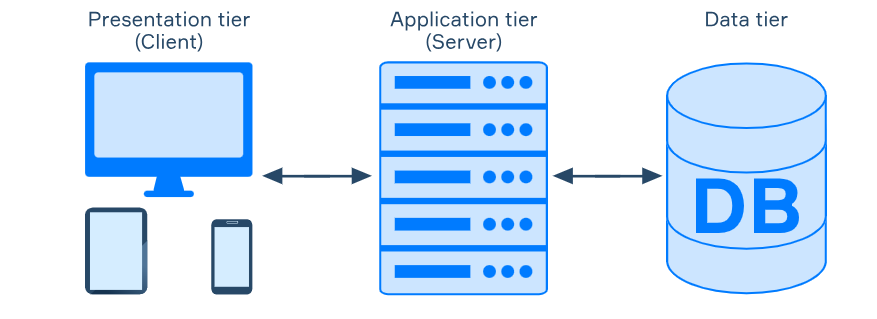
\includegraphics{Images/three tier architecture.png}
    \caption{Three tier architecture}\cite{three_Tier}
    \label{fig:three-tier}
\end{figure}

\subsection{Distributed view}
    \begin{figure}
        \centering
        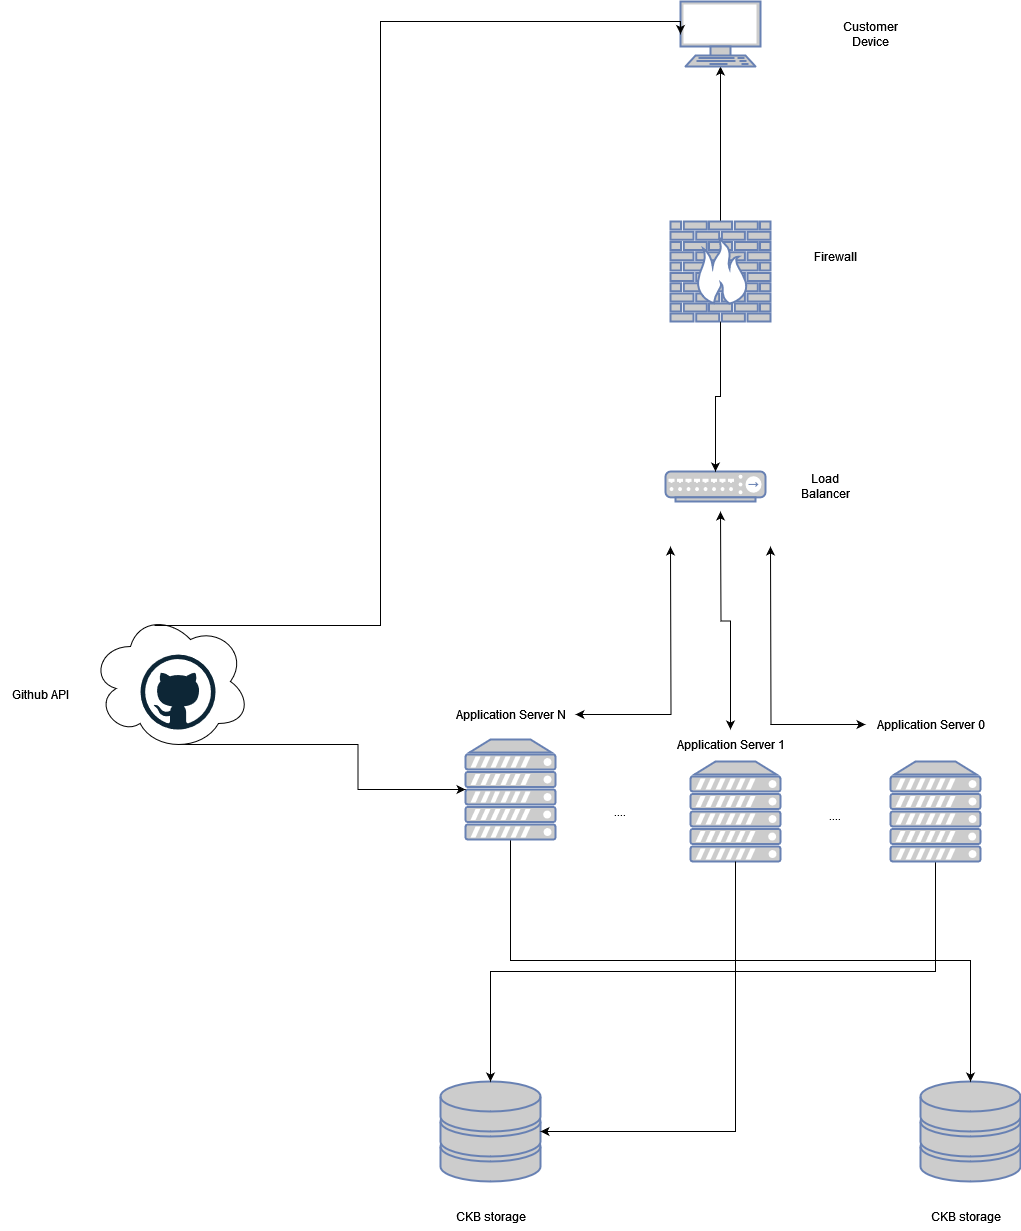
\includegraphics[width=\textwidth]{Images/DSV.drawio.png}
        \caption{Distributed view}
        \label{fig:enter-label}
    \end{figure}

\newpage
\section{Component view}
As mentioned for the platform we will use a three tier architecture. In figure \labelcref{fig:backend} it is possible to find the component view diagram of the platform. The back-end will implement an API which will be used by the web app (presentation layer). As you can see from the diagram, the data layer will also interact with the back-end, as will GitHub and the static analysis tool. The main components of the back-end are:
\begin{itemize}
    \item AuthenticationManager: provides the functionalities related to the authentication of the users to GitHub
    \item AccountManager: provides the functionalities related to the users general information and profile
    \item TeamManager: provides the functionalities related to the management of teams, necessary so students can participate in the battles.
    \item CompetitionStructureManager: This will implement the organizational part of the competition
    \item CompetitionEvaluationManager: Implements the evaluation of the competition. On contrast with the previous one, it is more dynamic because is triggered on every commit and it is also more computational intensive as it performs all the calculations needed for computing the score, the ranking and in order to assign the badges.
    \item DynamicAnalyser: implements the dynamic analysis tool that will run the test on the code submitted by the students. Because malicious users might try to exploit some vulnerability by providing malicious tests or code, we keep it separate from the previous.
    \item NotificationManager: Implements whats necessary so the platform can send notifications when needed
    \item Database: stores all the data of the app (Data Layer)
    \item API: The main purpose is to expose an API for the webApp, routing the incoming request to the appropriate internal component.

    For the front-end, the main component is:
        \begin{itemize}
            \item WebApp: The client app with which users will interact directly. Apart from the user interface it will contain some logic necessary to interact efficiently with the back-end REST API
        \end{itemize}
\end{itemize}

\newpage
\begin{figure}[!h]
    \centering
    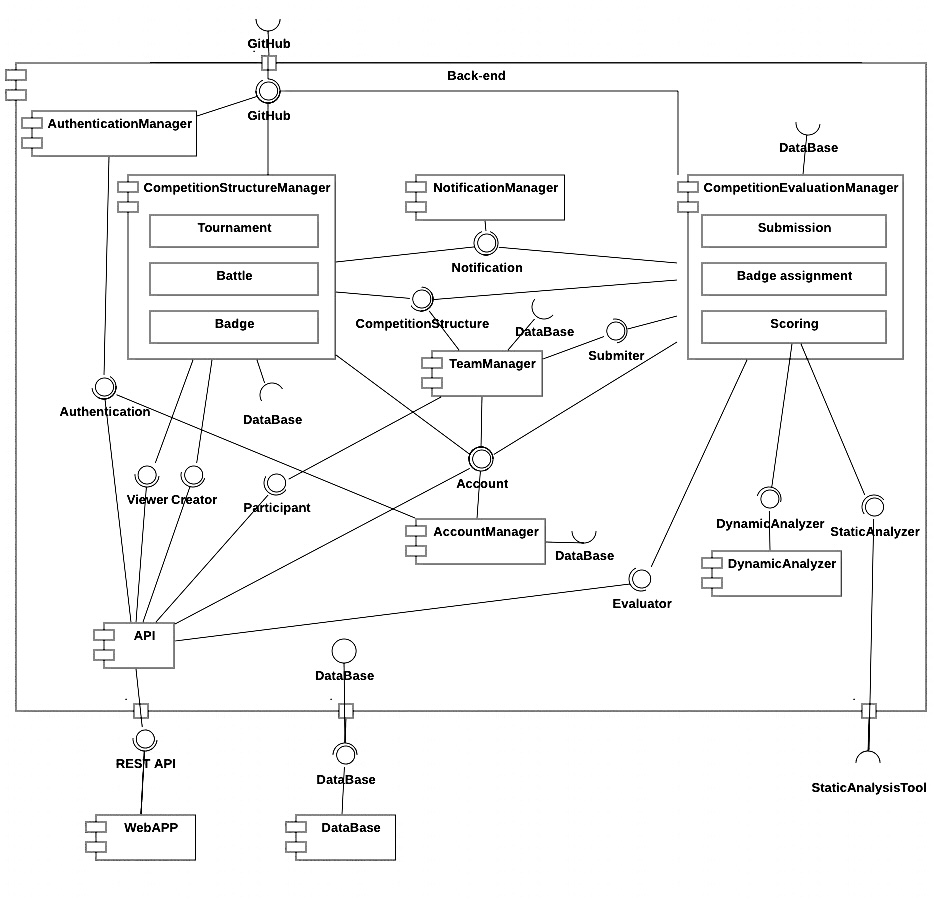
\includegraphics[width=\textwidth]{Images/Backend.jpeg}
    \caption{Component view}
    \label{fig:backend}
\end{figure}

\pagebreak
\section{Deployment view}
Here is showed the deployment view which is important because it describes the execution environment of the system but it also shows the topological distribution of the CKB application


\begin{figure}[!h]
    \centering
    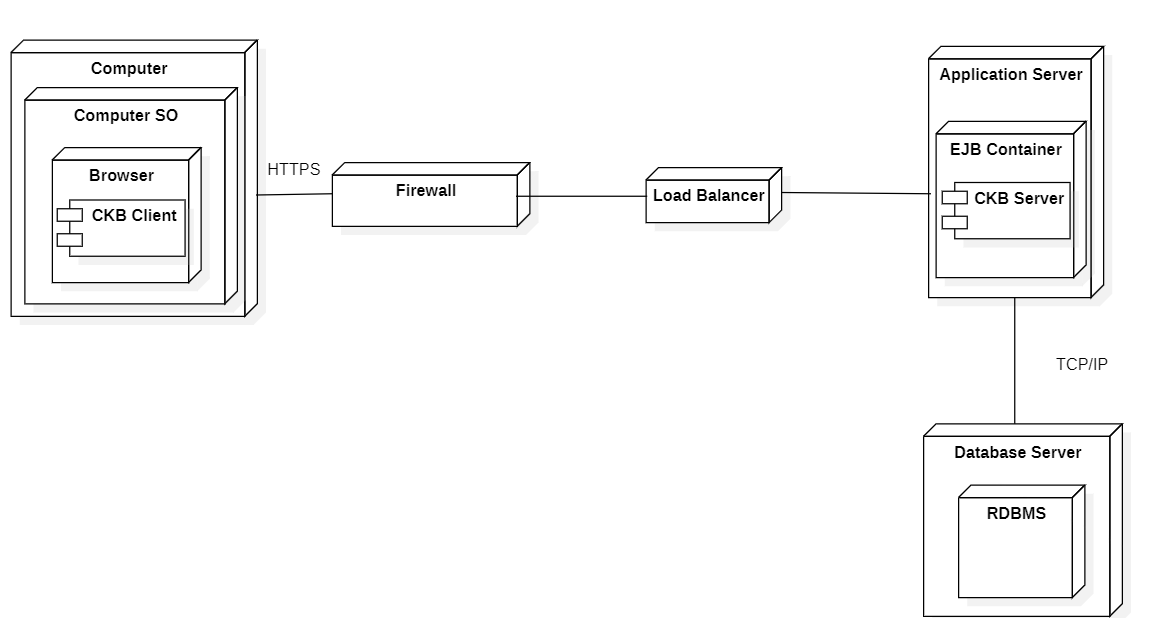
\includegraphics[width=\textwidth]{Images/Deployment_DIagram.png}
    \caption{Deployment view diagram}
    \label{fig:dep}
\end{figure}

The device SO is the one in which the browser is running from the browser it is possible to start the client-side app then every client request is processed by a firewall which is in charge of checking if some malicious request are sent to the server. A load balancer is a device useful for avoiding brute force attack to the server and, in general to not overload the server cpu capacities with a lot of request to process.The application server is able to manage the software architecture on the server-side then every change in the database is updated by the application server via TCP/IP.


\section{Runtime view}
\begin{enumerate}[label=\textbf{[UC\arabic*]}]
    \begin{figure}
    \item \textbf{User Registration}
        \centering 
        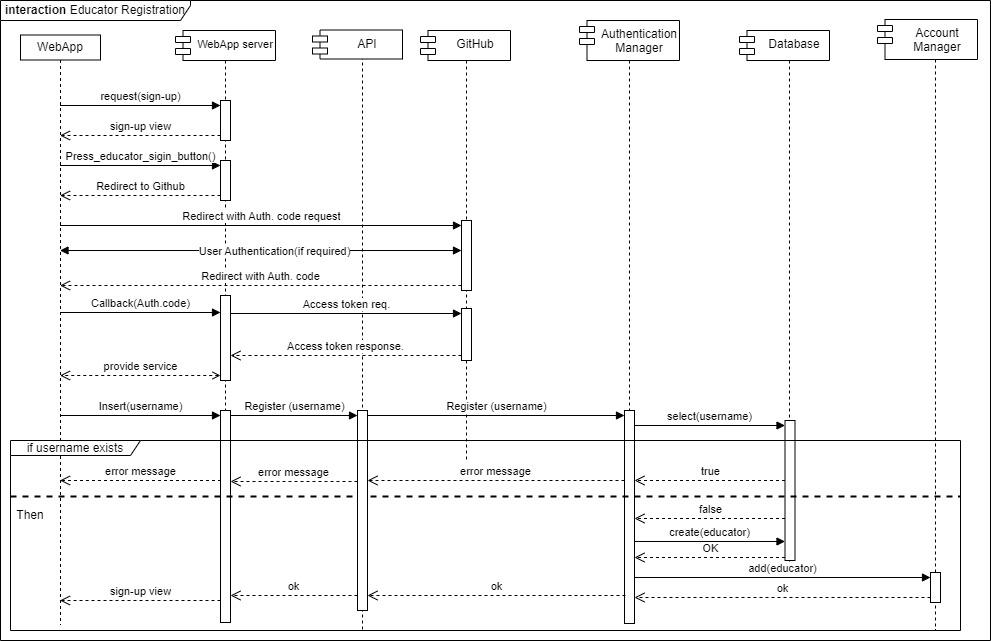
\includegraphics[width=\textwidth]{Images/User_registration.jpg}
        \caption{User Registration}
        \label{fig:enter-label}
        \raggedright The figure shows the process of the sign-in of the educator.
        Once it is sent the request to sign-up with GitHub, it will start the process of authentication, managed by the authentication manager. 
        GitHub handles authenticated requests after the application has obtained an access token.
        When the process of authentication is completed, the educator fills the educator profile form with the information needed to create the profile of the user who is signing up. 
        As soon as the form is submitted and sent to the authentication manager, it is asked to the database to check whether the username already exist in the platform. Then if the chosen username is new the database stores the information of the educator and the account manager adds the user to the table of educators.

        The process is the same for the student sign-up, however it is sent a different request from the browser to the webapp server. Another difference lies in storing student information that is separate from that of the educator. 
    \end{figure}

    \begin{figure}
    \item \textbf{User Login}
        \centering
        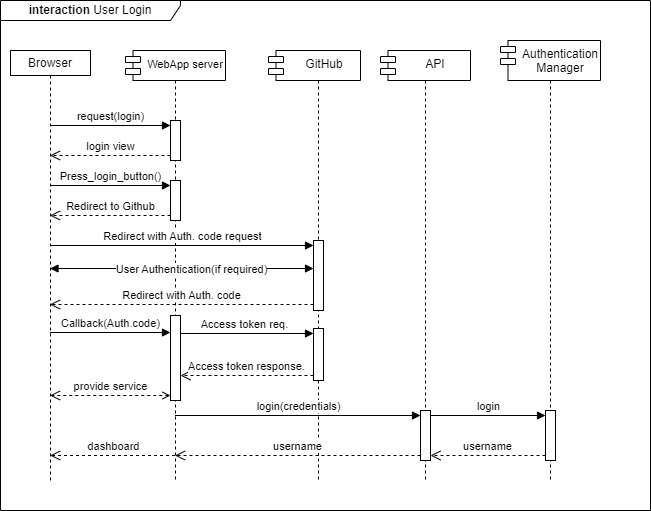
\includegraphics[width= \textwidth]{Images/User_login (1).jpg}
        \caption{User Login}
        \label{fig:enter-label}
        \raggedright The figure shows the process of login of a user. Since the information of both students and educators have been separately stored in the database, the process of login is the same for both of the two figures. 
        The login is managed by GitHub. Once the webapp has obtained the access token the webapp can check the credentials thanks to the authentication manager and let the user log to the platform.
    \end{figure}

    \begin{figure}
    \item \textbf{Tournament Creation}
        \centering
        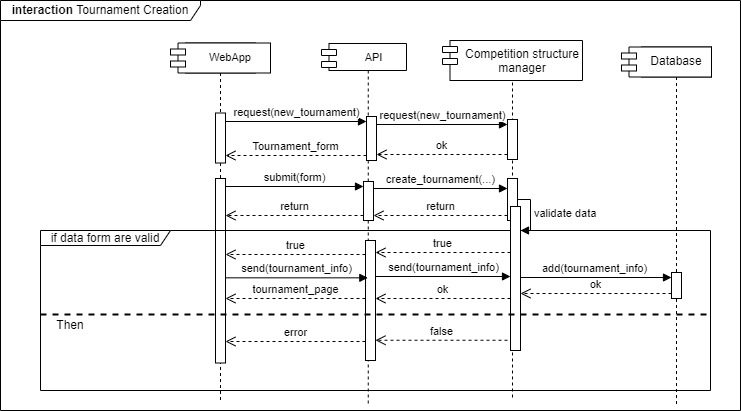
\includegraphics[width= \textwidth]{Images/Tournament_creation.jpg}
        \caption{Tournament Creation}
        \label{fig:enter-label}
        \raggedright This figure shows the process of the creation of the tournament. the user send to the WebApp  a request of creation of a new tournament. As a consequence the form is shown and it is filled with the tournament information. Then the competition structure manager is in charge of the validation of the information sent, if the information are valid they are inserted into the database.
    \end{figure}
    
    \begin{figure}
    \item \textbf{Battle Creation}
        \centering
        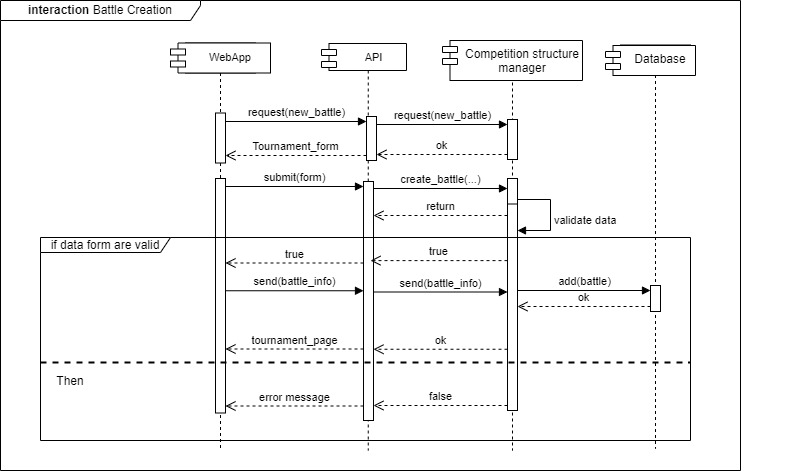
\includegraphics[width= \textwidth]{Images/Battle_creation.jpg}
        \caption{Battle Creation}
        \label{fig:enter-label}
        \raggedright The figure shows the process of the creation of a battle. As for the previous case, the user send to the WebApp  a request of creation of a new battle. So the form is shown and it is filled with the battle information. Then the competition structure manager is in charge of the validation of the information sent, if the information are valid they are insert into the database, in order to create the battle.
    \end{figure}
    
    \begin{figure}
    \item \textbf{Add collaborator}
        \centering
        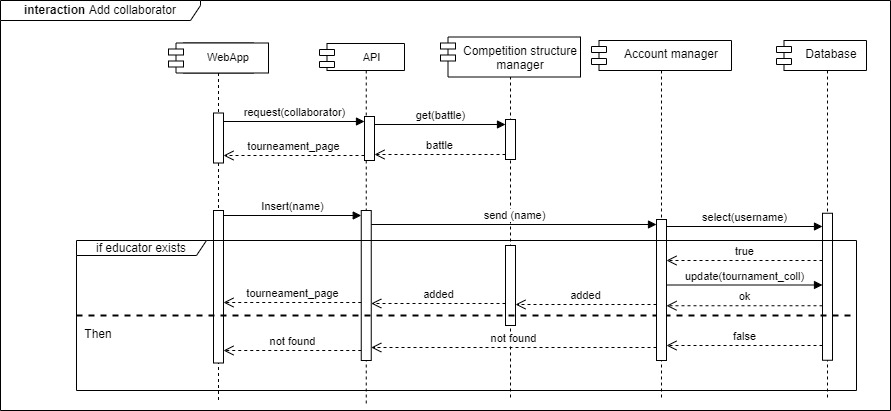
\includegraphics[width= \textwidth]{Images/Add_collaborator.jpg}
        \caption{Add collaborator}
        \label{fig:enter-label}
        \raggedright The figure shows the process of adding another educator to a tournament. The request is sent form the user to the competition structure manager which is in charge of return the tournament where the educator will be added.
        Then the user types the name of the user to add, then the account manager will request to the database to check whether the name inserted by the user is an educator. If yes the collaborator is added to the tournament collaborators.
    \end{figure}
    
    \begin{figure}
    \item \textbf{Team Creation}
        \centering
        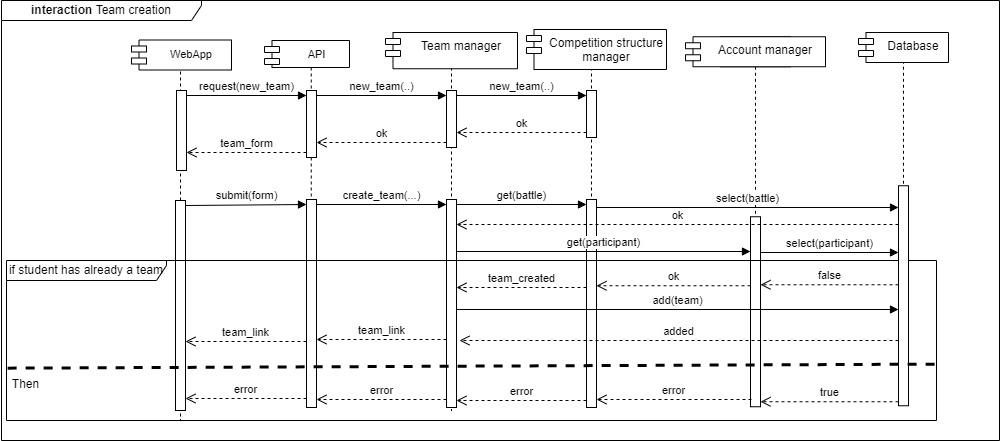
\includegraphics[width= \textwidth]{Images/Team_creation.jpg}
        \caption{Team Creation}
        \label{fig:enter-label}
        \raggedright The figure shows how a team is created. The student request the creation of a new team managed by the team manager. When the form is submitted, the team manager request to the competition structure manager the battle in order to associate the battle with it. In the end the competition structure manager has to check whether the user who request a team is a student already enrolled in a team. Once when it has been verified then it inserts the team into the database.
    \end{figure}
    
    \begin{figure}
    \item \textbf{Join Team}
        \centering
        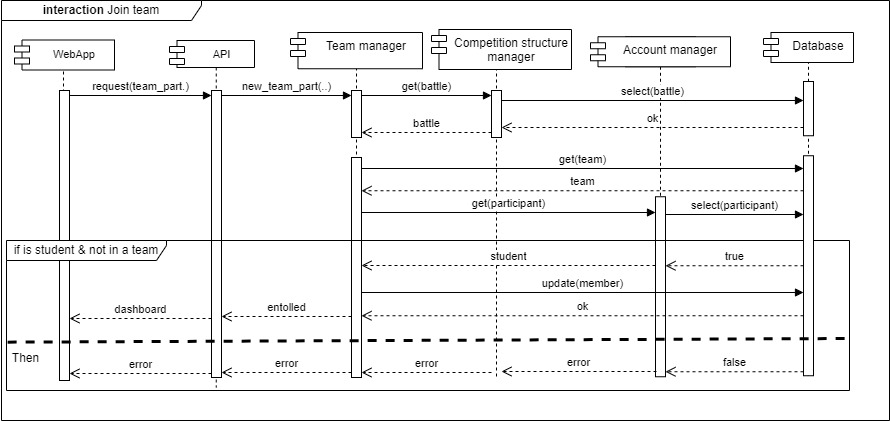
\includegraphics[width= \textwidth]{Images/Join_team.jpg}
        \caption{Join Team}
        \label{fig:enter-label}
        \raggedright The figure shows how a student that has already received a link can join a team. Once the link has been opened, the webapp send a request to the team manager to join the team. The manager asks the competition structure manager to get the battle information, then recover the information of the team associated to such battle. Then the manager check if the user is registered to the platform and and is not enrolled in other teams.
    \end{figure}
    
    \begin{figure}
    \item \textbf{Battle Begins}
        \centering
        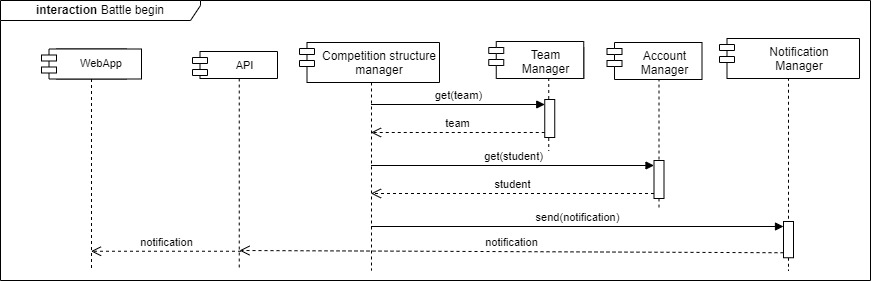
\includegraphics[width= \textwidth]{Images/Battle_begin.jpg}
        \caption{Battle Begins}
        \label{fig:enter-label}
        \raggedright The figure shows of the battle starts. As said in the RASD the battle starts as soon as the the enrollment deadline of the battle ended. Then the competition structure manager selects the students or the teams enrolled in such battle so that it can request to the notification manager to notify them.
    \end{figure}
    
    \begin{figure}
    \item \textbf{Code submission}
        \centering
        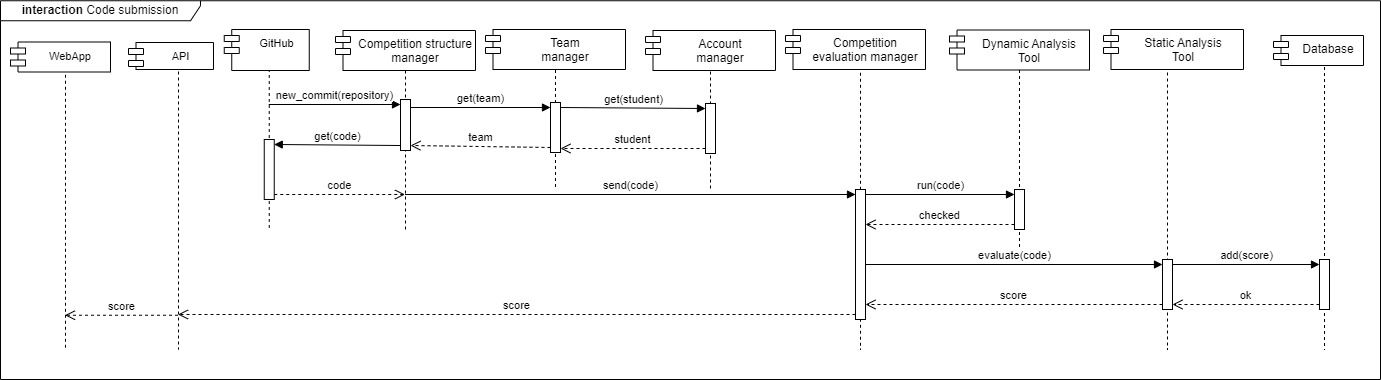
\includegraphics[width= \textwidth]{Images/Submits_code.jpg}
        \caption{Code submission}
        \label{fig:enter-label}
        \raggedright The figure shows the process of submission of a code from a certain team. The competition structure manager is triggered by GitHub as soon as a new commit has been done, as a consequence it looks for the team and its participants, in order to associate the code to the team. Then through a callback the manager gets the code so that it can be sent to the competition evaluation manager which is in charge of request to the dynamic analysis tool to check the code. Once the code has been checked the manager request the evaluation to the static analysis tool. The resulting score will be added to the database and sent to the webapp.
    \end{figure}

    \begin{figure}
    \item \textbf{The battle ends}
        \centering
        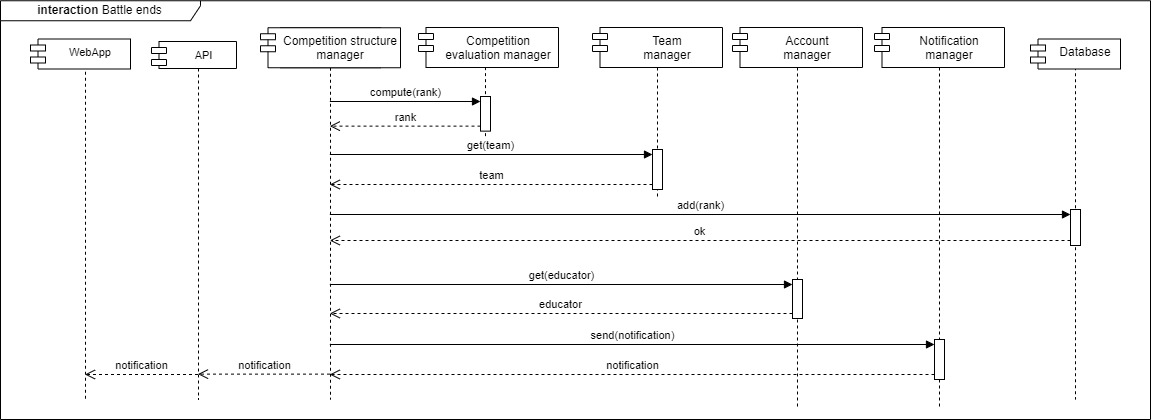
\includegraphics[width= \textwidth]{Images/Battle_ends.jpg}
        \caption{The battle ends}
        \label{fig:enter-label}
        \raggedright The figure shows how is it managed the end of a battle. The competition structure manager ask the competition evaluation manager to compute the rank of the battle, than request the team manager to get the team in order to associate the ranks to the teams and store it in the database. In the end it ask the notification manager to notifies students about the new rank.
    \end{figure}
    
    \begin{figure}
    \item \textbf{Code Evaluation}
        \centering
        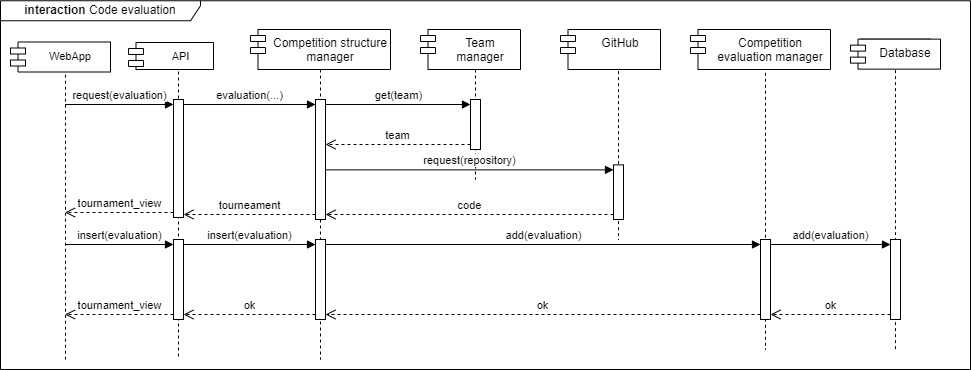
\includegraphics[width= \textwidth]{Images/Code_Evaluation.jpg}
        \caption{Code Evaluation}
        \label{fig:enter-label}
        \raggedright The figure shows the process of manual evaluation done by the educators at the end of the tournament,if necessary. The consolidation phase started. The webapp request the competition structure manager for a manual evaluation, as a consequence the manager request the team to the team manager and the code from GitHub which retrieves it through the repository. Then the user can inset his evaluation in the platform which will be sent to the competition structure manager and the competition evaluation manager and finally stored in the database.
    \end{figure}

    \begin{figure}
    \item \textbf{Publish Final Rank}
        \centering
        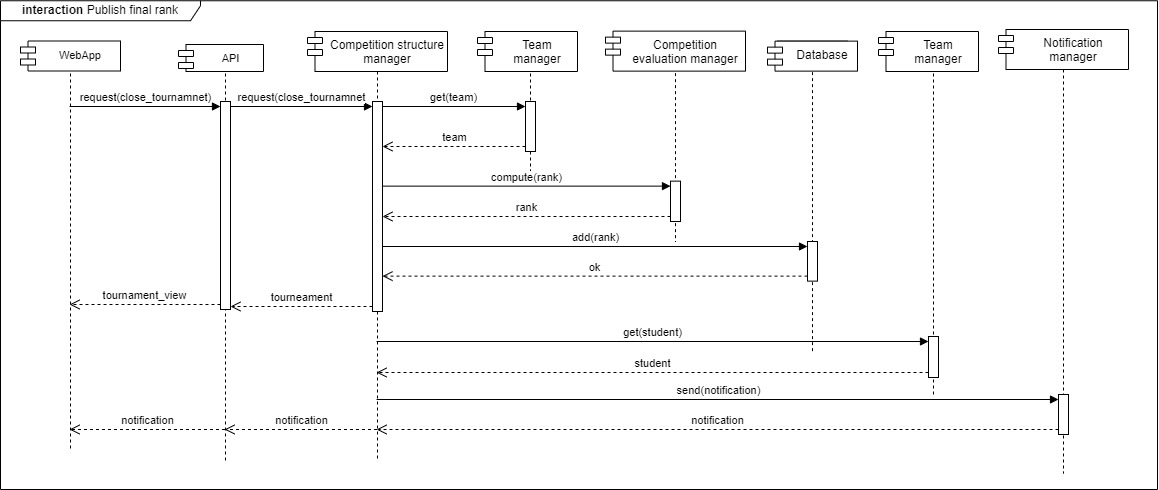
\includegraphics[width= \textwidth]{Images/Publish_Final_Rank.jpg}
        \caption{Publish Final Rank}
        \label{fig:enter-label}
        \raggedright The figure shows the process of closure of the tournament. When the educator closes the tournament, the competition structure manager takes care of recovering the name of the team and asks the competition evaluation manager to calculate the final rank and so updates the rank in the database.
        After that the competition structure manager is in charge of notify the student about the final rank update. Asks the account manager the name of the student who will receive the notification from the notification manager.
    \end{figure}

    \begin{figure}
    \item \textbf{See Profile}
        \centering
        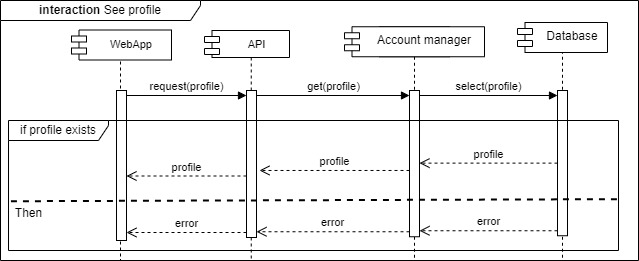
\includegraphics[width= \textwidth]{Images/See_Profile.jpg}
        \caption{See Profile}
        \label{fig:enter-label}
        \raggedright The figure shows how the user can look for a profile of a user in the platform. As soon as the name is searched, is sent a request of getting a profile to the account manager, which ask the database to check whether the name is a user of the platform.
    \end{figure}
    \begin{figure}
    \item \textbf{Badge Creation}
        \centering 
        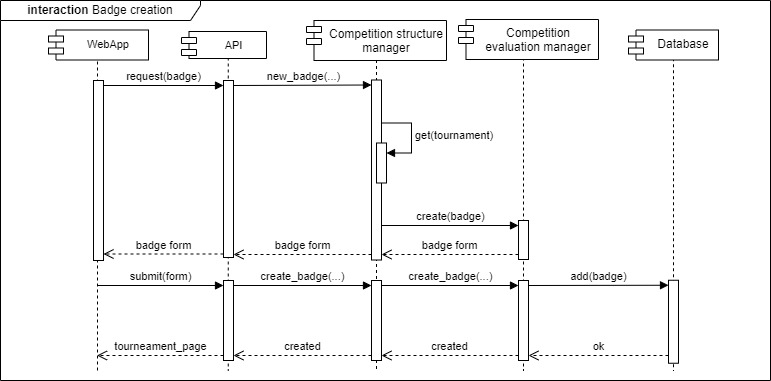
\includegraphics[width= \textwidth]{Images/Badge_Creation.jpg}
        \caption{Badge Creation}
        \label{fig:enter-label}
        \raggedright The figure shows the creation of a badge. The request is sent to the competition structure manager which gets the tournament associated to the badge. When the form of the badge has been submitted, the competition structure manager forward the request of creation of the badge to the competition evaluation manager and then the badge is added to the database.
    \end{figure}
\end{enumerate}
\pagebreak

\section{ Component interfaces}

    \subsubsection{WebApp server}
    \begin{itemize}
        \item request(sign-up)
        \item press educator sigin button()
        \item callback(Auth.code)
        \item request(login)
        \item Press login button()
    \end{itemize}
    
    \subsubsection{GitHub}
    \begin{itemize}
        \item redirect with Auth. code request
        \item access token req.
        \item request(repository)
    \end{itemize}
    
    \subsubsection{API}
    \begin{itemize}
        \item register (username)
        \item login(credentials)
        \item login
        \item request(new tournament)
        \item submit(form)
        \item send(tournament info)
        \item request(new battle)
        \item send(battle info)
        \item request(collaborator)
        \item insert(name)
        \item request(new team)
        \item request(evaluation)
        \item insert(evaluation)
        \item request(close tournament)
        \item request(profile)
        \item request(badge)
    \end{itemize}
    
    \subsubsection{AuthenticationManager}
    \begin{itemize}
        \item register (username)
    \end{itemize}
    
    \subsubsection{CompetitionStructureManager}
    \begin{itemize}
        \item request(new tournament)
        \item send(tournament info)
        \item validate data
        \item request(new battle)
        \item get(battle)
        \item new team(...)
        \item request(team part.)
        \item new get(student)commit(repository)
        \item evaluation(...)
        \item insert(evaluation)
        \item request(close tournament)
        \item new badge(...)
        \item get(tournament)
        \item create badge(...)
    \end{itemize}
    
    \subsubsection{CompetitionEvaluationManager}
    \begin{itemize}
        \item send(code)
        \item compute(rank)
        \item add(evaluation)
        \item create(badge)
        \item create badge(...)
    \end{itemize}
    
    \subsubsection{NotificationManager}
    \begin{itemize}
        \item send(notification)
    \end{itemize}
    
    \subsubsection{TeamManager}
    \begin{itemize}
        \item new team(...)
        \item create team(...)
        \item new team part(...)
        \item get(team)
    \end{itemize}
    
    \subsubsection{AccountManager}
    \begin{itemize}
        \item select(username)
        \item add(educator)
        \item add(student)
        \item send (name)
        \item get(participant)
        \item get(student)
        \item get(educator)
        \item get(profile)
    \end{itemize}
    
    \subsubsection{DynamicAnalyzer}
    \begin{itemize}
        \item run(code)
    \end{itemize}
    
    \subsubsection{StaticAnalysisTool}
    \begin{itemize}
        \item evaluate(code)
    \end{itemize}
    
    \subsubsection{Database}
    \begin{itemize}
        \item create(educator)
        \item create(student)
        \item add(tournament info)
        \item add(battle)
        \item select(username)
        \item update(tournament coll)
        \item select(battle)
        \item select(participant)
        \item add(team)
        \item get(team)
        \item update(member)
        \item add(score)
        \item add(rank)
        \item add(evaluation)
        \item select(profile)
        \item add(badge)
    \end{itemize}

\pagebreak
\section{Selected architectural styles and patterns}
\subsection{3-tier Architecture}
The architectural style that is used is the 3-tier architecture style because it provides many benefits the main one is the modularization in three independent layers:

            \begin{itemize}
                \item  The \textbf{ web server}:is the presentation tier and provides the user interface.This is usually a web page or a web site.The content can be static or dynamic, and is usually developed using HTML, CSS and Javascript.
                \item The \textbf{application server}:it is the middle tier, implementing the business logic.
                \item The \textbf{database server}:it is the backend tier of a web application. It runs on DBMS, such as MySQL.
            \end{itemize}

\subsection{Model View Controller Pattern }
The CKB is basically a web application that allows users to have access to the CKB features.So The MVC pattern is the the best choice to implement the application:

    \begin{itemize}
        \item  \textbf{Model}:it manages the data, logic and rules of the application.
        \item  \textbf{View}:representation of information such as a chart. Multiple views of the same information are possible, such as a bar chart for management and a tabular view for accountants. 
        \item   \textbf{Controller}:it accepts input and converts it into commands for Model and view.
    \end{itemize}
    
The tasks division between these three elements provide a  strong decoupling which gives some benefits such as reliability, re usability .      

\subsection{Facade Pattern}
The facade pattern is a software design pattern that is useful for implementing the requests dispatching.In fact, the facade is an object that hides the more complex underlying. it improves the readability and usability of a software library by masking interaction with more complex components behind a single  API. it provides a context-specific interface to more generic functionality and it serves as a launching point for a broader refactor of monolithic or tightly-coupled systems in favor of more loosely-coupled code.
 
\section{Other design decisions}
In this section are explained some design decisions that have been taken in order to make the system work

\subsection{Availability}
The concept of Load Balancing has been introduced to design a system which is highly available and to be able to manage an high amount of request at the same time.it's also important to have some sort of replication to avoid a single point of failure.

\subsection{Data Storage}
The data storage is managed by using a database to store  the personal data of educator and students. Moreover, are used some additional data structure to have better query performances 

\subsection{Security}
The security is managed by means of a firewall that is necessary to filter some cyber attacks.




%------------------------------------------------------------------------------------------------------------------------------------------------
\clearpage
{{\chapter{User Interface Design}}}
\label{sect:ui}
\begin{figure}[!h]
    
        \centering
        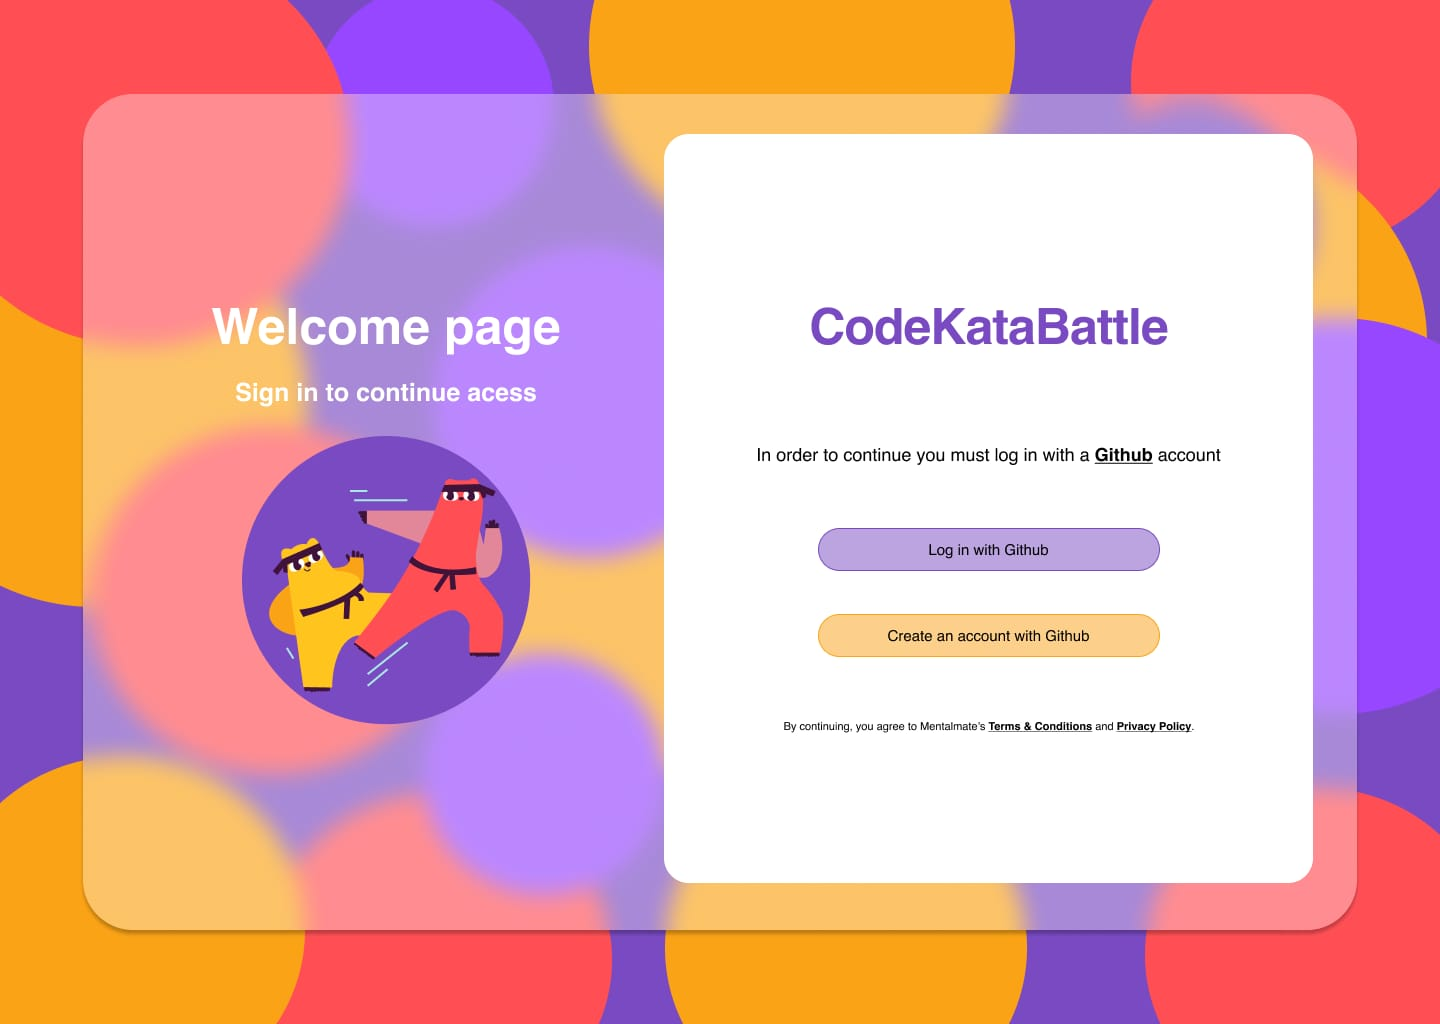
\includegraphics[width= 13cm]{Images/login_interface.jpg}
        \caption{User login}
        \label{fig:enter-label}
    \end{figure}


\begin{figure}[!h]
    
        \centering
        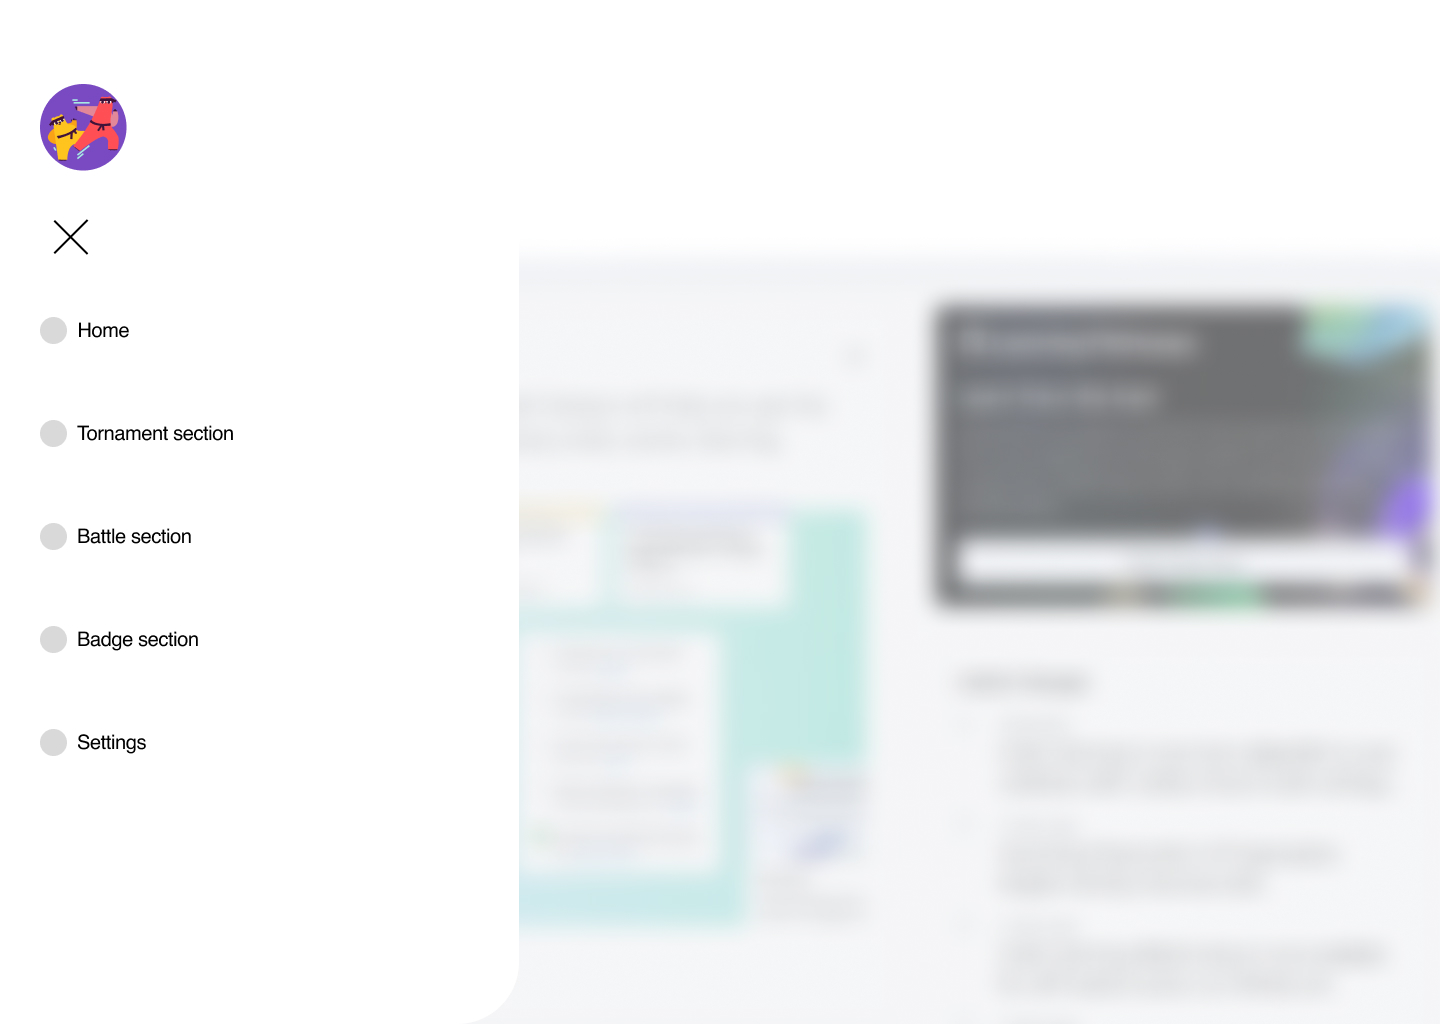
\includegraphics[width= 13cm]{Images/select_interface.jpg}
        \caption{selection bar}
        \label{fig:enter-label}
\end{figure}


\begin{figure}[!h]
    
        \centering
        
\includegraphics[width= 13cm]{Images/dashboard_access.jpg}
        \caption{menu}
        \label{fig:enter-label}
\end{figure}


%------------------------------------------------------------------------------------------------------------------------------------------------
\clearpage
{{\chapter{Requirements Traceability}}}
\label{sect:requirements}
\section{External Interface Requirements}
\subsection{User Interfaces}
In this section is presented the UI of the web platform here are presented two type of user interfaces the one for the educator and the one for the student. The first one has the possibility to create tournaments and battles.
The second one has the possibility to compete inside a tournament and to receive some badges that shows the abilities that the student himself has consolidated by using the platform.Both the two types of users  need to insert their credentials to have access to the platform.Moreover a mechanism of forgot password it's needed just in case they lose their credentials. 
\subsection{Hardware Interfaces}
Our platform is a web app, as a consequence, it does not require any specific hardware interface except for computer and any other device with web browser.
\subsection{Software Interfaces}
In order to work the system needs some software  interfaces. Here they are listed in detail:
    \begin{itemize}
        \item Github API:In order to interact with github, for user login and registration as well as to create and manage repositories;
        \item Calendar API:it's useful to suggest to the user what battle it's going to happen;
        %\item Email notification:This API is useful because the user will receive a notification via email when a battle starts;
        \item Static analysis tool API: To evaluate the submitted code, we will send a request to the static tool with the code and then we expect an answer with the assigned score.
    \end{itemize}
\subsection{Communication Interfaces}
The user uses the internet connection to have access to the platform,to communicate with other user inside the platform and for pushing and pulling the code on github.The platform must be HTTPS compliant in order to work on the web properly and to be safe. 

\section{Functional Requirements}
%Definition of use case diagrams, use cases and associated sequence/activity diagrams, and mapping on requirements


\textbf{Sign up and log in}
\begin{enumerate}[label={[R\arabic*]}]
    
    \item The System allows users\footnote{users is used to refer to students and educators} to register by providing their personal information (Full Name, etc.), a valid email address and a password.
    \item The System allows registered user to log in
    \\  \\  \textbf{Tournament and battles management}
    \item The System allows Educators to create/modify a battle upload the code kata (description and software project, including test cases and build automation scripts)
    \item The System allows to create/modify/terminate a tournament by selecting the existing battles, setting the minimum and maximum number of students per group, the registration and final submission deadline.
    \item The System allows an educator to give or deny permission to his colleagues to modify a tournament.
    \item The System must notify subscribed user about upcoming battles and deadlines.
    \\  \\  \textbf{Student's teams}
    \item The System allows students to create a team
    \item The System allows students to invite other students into one of their teams
    \item The System allows students to join a new team which they were invited
    \\  \\  \textbf{Scoring and ranking}
    \item The system allows educators to define the scoring criteria for a specific battle which they have permissions to
    \item The system maintains and computes the scores of each battle
    \\ \\  \textbf{Badges}
    \item Educators can create a badge and a set of rules associated with that badge
    \item The system assigns the badges that are created by educators as a reward for the rules they fulfill
    \item The system shows the badges that are assigned to students

    \\  \\  \textbf{Tournament and battles participation}
    \item The System creates a repository on GitHub containing the code kata right after the registration deadline
    \item The system sends the link to all the enrolled students after creating the repository with the code kata
    \item The System receives notifications from GitHub regarding the students registered repositories commits
    \item The System pulls the repository after receiving a notification for that repository before the deadline of that battle
    \item The System runs the appropriate test on the new code after every pull of the repository
    \item The System calculate and update the team's score for that battle after rerunning the tests
    \\  \\  \textbf{Tournament and battles consolidation}
    \item The system updates the personal tournament score for each student enrolled in the tournament right after the battle ends
    \item The system allows educators to manually evaluate the code after the deadline
    \item The system  allows educators to finish the consolidation stage after completely performing the manual evaluation
    \item The system computes the final ranking of the tournament immediately after consolidation finishes
    \item The system  sends a notification about the tournament's termination to students 
\end{enumerate}

\subsection{Use cases Diagram}

\begin{wrapfigure}
    \centering
    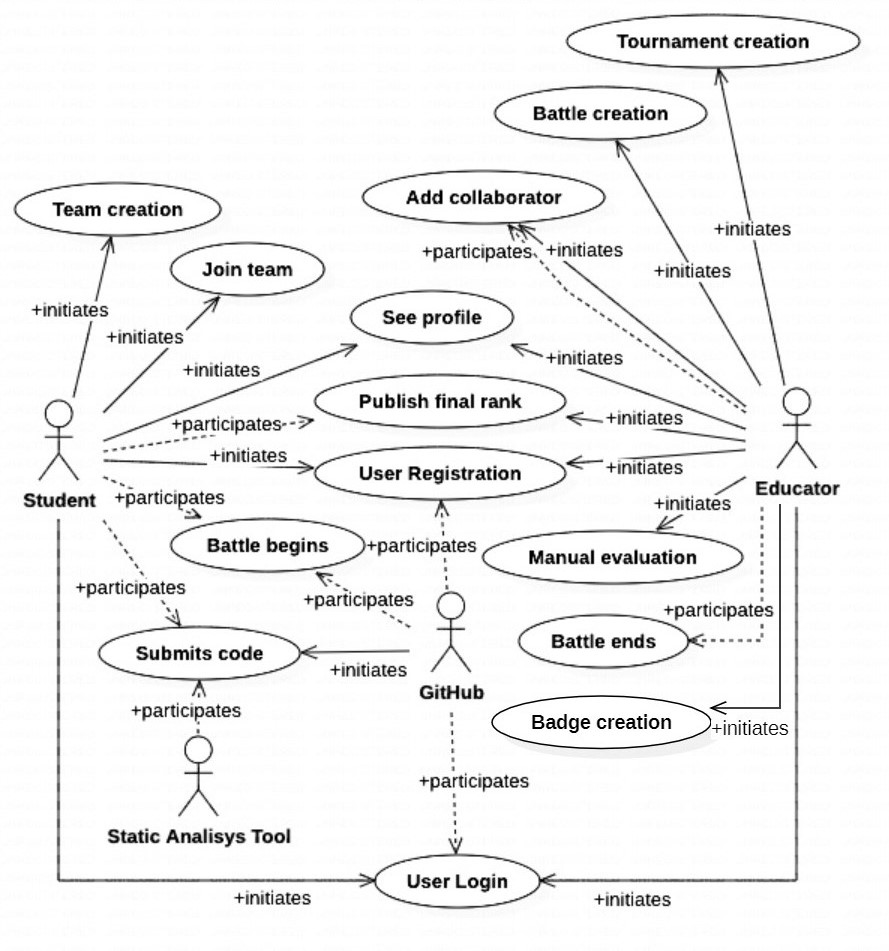
\includegraphics[width=15cm]{Images/ucd.jpg}
    \caption{Use cases diagram}
    \label{fig:enter-label}
\end{wrapfigure}

\subsection{Use cases}

\begin{enumerate}[label=\textbf{[UC\arabic*]}]
    \item \textbf{-User Registration}
    \\ \begin{tabular}{|l|p{11cm}|}
        \hline
        Name & User Registration \\
        \hline
        Actors & \begin{itemize}
                    \item user
                    \item GitHub
                \end{itemize} \\
        \hline
        Entry Condition & The user has opened the CKB platform\\
        \hline
        Event flow & \begin{enumerate} 
            \item The user press the button Sign-in
            \item The system redirect the user on GitHub to link their account to the platform
            \item The system shows a form to compile
            \item The user compile the form by adding a username
            \item The user press the button 'Register' to complete the registration
            \item The platform shows the login view
        \end{enumerate}\\
        \hline
        Exit condition & The user has successfully registered to the platform \\
        \hline
        Exception & \begin{enumerate} [label={}, leftmargin=0.25cm ]
            \item (d) There already exist a user with those credentials.
        \end{enumerate}  \\
        \hline            
    \end{tabular}
\newpage
    
 \item \textbf{-User Login}  
    \\ \begin{tabular}{|l|p{11cm}|}
        \hline
        Name & User Login\\
        \hline
        Actors & \begin{itemize}
                    \item user
                    \item GitHub
                \end{itemize} \\
        \hline
        Entry Condition & The user has opened the CKB platform\\
        \hline
        Event flow & \begin{enumerate}
            \item The user press the button Log-in
            \item The System redirect the user to GitHub platform to let him login to it, and checks the credentials
            \item The user is redirected to the platform with an access token
            \item The system shows the profile information
            \item The user presses the button 'Login'
            \item The platform shows the dashboard
        \end{enumerate}\\

        \hline
        Exit condition & The user has successfully accessed the service \\

        \hline
        Exception & \begin{enumerate} [label={}, leftmargin=0.25cm ]
            \item (c) The token is not valid. The platform will return to the entry condition
        \end{enumerate} \\ 
        \hline                
    \end{tabular}
    \pagebreak
   

\item  \textbf{-Tournament creation}
\\\begin{tabular}{|l|p{11cm}|}
        \hline
        Name & Tournament creation \\
        \hline
        Actors & \begin{itemize}
                    \item educator
                \end{itemize} \\
        \hline
        Entry Condition & The Educator is logged to the CKB platform\\
        \hline
        Event flow & \begin{enumerate}
            \item The educator goes to the tournament section
            \item The educator press the button to create a new tournament
            \item The system shows the educator the form to compile
            \item The educator fills the form with the information about the tournament:
            name, main context, enrolment deadline
            \item The educator press the button to submit the form
        \end{enumerate}\\
        \hline
        Exit condition & The educator has successfully created the tournament and returns to the tournament section  \\
        \hline
        Exception & \begin{enumerate} [label={}, leftmargin=0.25cm ]
            \item (d) The educator did not fill all the field of the form or they are not valid. The system will warn the user.
        \end{enumerate} \\
        \hline            
    \end{tabular}

\newpage
 \item \textbf{-Battle creation}
    \\ \begin{tabular}{|l|p{11cm}|}
        \hline
        Name & Battle Creation \\
        \hline
        Actors & \begin{itemize}
                    \item educator
                \end{itemize} \\
        \hline
        Entry Condition & The Educator is logged to the CKB platform and he already created a tournament\\
        \hline
        Event flow & \begin{enumerate}
            \item The educator goes to the tournament where he want to add the battle
            \item The educator press the button to create a new battle
            \item The system shows the educator the form to compile
            \item The educator fills the form with the information about the battle with the following information: battle name, code template, registration deadline, final submission deadline, sets minimum and maximum number of students per group that can participate in that battle and the scoring criteria for that battle
            \item The educator press the button to submit the form
        \end{enumerate}\\
        \hline
        Exit condition & The educator has successfully created the new battle and returns to the tournament main page \\
        \hline
        Exception & \begin{enumerate} [label={}, leftmargin=0.25cm ]
            \item (d) The educator did not fill all the field of the form or they are not valid. The system will warn the user. 
        \end{enumerate}\\
        \hline            
    \end{tabular}

\item \textbf{-Add collaborator}
    \\ \begin{tabular}{|l|p{11cm}|}
        \hline
        Name & Add collaborator\\
        \hline
        Actors & \begin{itemize}
                    \item educator
                \end{itemize} \\
        \hline
        Entry Condition & The educator is logged to the CKB platform and he is in the tournament section\\
        \hline
        Event flow & \begin{enumerate}
            \item The educator select the tournament
            \item The educator press the button to share the control of a tournament
            \item The system shows the educator a bar where to search other educators
            \item The educator can choose the other educators
            
        \end{enumerate}\\
        \hline
        Exit condition & The educator has successfully shared the access to the tournament control  \\
        \hline
        Exception & \begin{enumerate} [label={}, leftmargin=0.25cm ]
            \item (d) The educator did not make the correct choice
        \end{enumerate} \\
        \hline            
    \end{tabular}

\newpage
\item  \textbf{-Team creation}
    \\ \begin{tabular}{|l|p{11cm}|}
        \hline
        Name & Team creation \\
        \hline
        Actors & \begin{itemize}
                    \item student
                \end{itemize} \\
        \hline
        Entry Condition & The student is logged to the CKB platform and is enrolled into a tournament\\
        \hline
        Event flow & \begin{enumerate}
            \item The student goes to tournament section and selects the tournament
            \item The student select the battle for which create the team
            \item The student press the button create a team
            \item The system shows the student the form to compile
            \item The student fills the form with the information about the team: team name
            \item The system generate the link of the team 
            \item The student shares the link of the team with his friends
        \end{enumerate}\\
        \hline
        Exit condition &  The link team is successfully generated \\
        \hline
        Exception & \begin{enumerate} [label={}, leftmargin=0.25cm ]
            \item (c) The student has already created a team for that battle
        \end{enumerate} \\
        \hline            
    \end{tabular}

\item  \textbf{-Join team}
    \\ \begin{tabular}{|l|p{11cm}|}
        \hline
        Name & Join team  \\
        \hline
        Actors & \begin{itemize}
                    \item student
                \end{itemize} \\
        \hline
        Entry Condition & The student has the link to join a team\\
        \hline
        Event flow & \begin{enumerate}
            \item The student opens the link received
            \item The system checks the student's credentials
            \item The student press the button 'join the team'
            \item The system checks if the team is not full and that the student is not already enrolled in the battle
            \item The system redirect the student into the team dashboard
        \end{enumerate}\\
        \hline
        Exit condition &   The student has correctly joined the team \\
        \hline
        Exception & \begin{enumerate} [label={}, leftmargin=0.25cm ]
            \item (b) The student is not logged in, he will be redirect to the log in page
            \item (d) The system returns an error message
        \end{enumerate}\\ 
        \hline            
    \end{tabular}
\newpage
    \item  \textbf{-Battle begins}
    \\ \begin{tabular}{|l|p{11cm}|}
        \hline
        Name & Battle begins \\
        \hline
        Actors & \begin{itemize} 
                    \item student
                    \item GitHub
                \end{itemize} \\
        \hline
        Entry Condition & The enrollment deadline of the battle ended\\
        \hline
        Event flow & \begin{enumerate}
            \item The system creates a GitHub repository by using the appropriate API call for every enrolled team enrolled
            \item The system sends a notification to the students enrolled to the battle with the link to the specifically created repository for them to fork
        \end{enumerate}\\
        \hline
        Exit condition &   The code is available to all the students participating\\
        \hline
        Exception & \begin{enumerate} [label={}, leftmargin=0.25cm ]
            \item (b) The notification is not correctly sent, the system will retry to send it later.
        \end{enumerate}\\ 
        \hline            
    \end{tabular}

 \item  \textbf{-Submits code}
    \\ \begin{tabular}{|l|p{11cm}|}
        \hline
        Name & Student pushes the code \\
        \hline
        Actors & \begin{itemize}
                    \item student
                    \item GitHub
                    \item Static analysis tool
                \end{itemize} \\
        \hline
        Entry Condition & The student has forked to the git hub repository provided by the platform and set up the automated workflow. The student has committed the code into their GitHub repository\\
        \hline
        Event flow & \begin{enumerate}
            \item The system is triggered by GitHub about a new commit
            \item The system dynamically evaluates the code by running the test on it.
            \item The system send the code to the static analysis tool 
            \item The system receives the evaluation by the tool
            \item The system updates the score of the team.
        \end{enumerate}\\
        \hline
        Exit condition &   The scoring rank is correctly updated\\
        \hline
        Exception & \begin{enumerate} [label={}, leftmargin=0.25cm ]
             \item (a) The repository is not a fork of a code kata team, the system will ignore it and log it.
            \item (a) The system is triggered after the deadline of the battle, it will not evaluate the code and send a notification to the team warning them 
           
        \end{enumerate}\\ 
        \hline            
    \end{tabular}
\newpage
    \item  \textbf{-The battle ends}
    \\ \begin{tabular}{|l|p{11cm}|}
        \hline
        Name & The battle ends \\
        \hline
        Actors & \begin{itemize}
                    \item educator
                \end{itemize} \\
        \hline
        Entry Condition & the battle deadline has expired \\
        \hline
        Event flow & \begin{enumerate}
            \item The system creates the rank of the battle
            \item The system sends a notification the the educators enrolled into the battle about the end of it
        \end{enumerate}\\
        \hline
        Exit condition & The ranking is available on the platform \\
        \hline
        Exception & \begin{enumerate} [label={}, leftmargin=0.25cm ]
            \item (b) The notification is not correctly sent, the system will notify it and retry to send it
        \end{enumerate}\\ 
        \hline            
    \end{tabular}

        \item  \textbf{-Code evaluation}
    \\ \begin{tabular}{|l|p{11cm}|}
        \hline
        Name & The code is evaluated \\
        \hline
        Actors & \begin{itemize}
                    \item educator
                \end{itemize} \\
        \hline
        Entry Condition & The tournament ended, the consolidation phase started and the educator is logged to the CKB platform\\
        \hline
        Event flow & \begin{enumerate}
            \item The educator goes to the tournament section
            \item The educator select the tournament which needs a manual evaluation
            \item The educator reads the sources produced by the teams
            \item The educator assign a score to each student enrolled to the battle
        \end{enumerate}\\
        \hline
        Exit condition &  The system stores the score provided by the educator\\
        
        \hline            
    \end{tabular}
\newpage
        \item  \textbf{-Publish final rank}
    \\ \begin{tabular}{|l|p{11cm}|}
        \hline
        Name & Final rank made available \\
        \hline
        Actors & \begin{itemize}
                    \item student
                    \item educator
                \end{itemize} \\
        \hline
        Entry Condition & The tournament is in consolidation phase, the educator is logged to the CKB platform \\
        \hline
        Event flow & \begin{enumerate}
            \item The educator goes to the tournament section
            \item The educator selects the tournament to close
            \item The educator press the button 'close the tournament'
            \item The system computes the final rank for each student enrolled into the tournament
            \item The system notifies the student about the availability of the rank
            \item The system checks among the participating students who satisfied the badges requirement
            \item The system assign the badge to the students
        \end{enumerate}\\
        \hline
        Exit condition &  The final rank is published, and badges has been assigned \\
        \hline
        Exception & \begin{enumerate}  [label={}, leftmargin=0.25cm ]
            \item (c) If any student does not have a manual evaluation and it was required then an error message will be shown.
            \item (e) The notification is not correctly sent, the system will notify it and retry to send it
        \end{enumerate}\\ 
        \hline            
    \end{tabular}


        \item  \textbf{-See profile}
    \\ \begin{tabular}{|l|p{11cm}|}
        \hline
        Name & see profile \\
        \hline
        Actors & \begin{itemize}
                    \item user
                \end{itemize} \\
        \hline
        Entry Condition &  The user is logged to the CKB platform\\
        \hline
        Event flow & \begin{enumerate}
            \item The user search the name of the student
            \item The system shows the list
            \item The user selects the Student
        \end{enumerate}\\
        \hline
        Exit condition & The platform shows the rank of the selected student  
        \\
        \hline
        Exception & \begin{enumerate} [label={}, leftmargin=0.25cm ]
            \item (a) The person searched  does not match with any user in the system. It shows a no student found message
        \end{enumerate}\\ 
        \hline            
    \end{tabular}

\newpage


 \item \textbf{-Badge creation}
    \\ \begin{tabular}{|l|p{11cm}|}
        \hline
        Name & Badge Creation \\
        \hline
        Actors & \begin{itemize}
                    \item educator
                \end{itemize} \\
        \hline
        Entry Condition & The educator is logged to the CKB platform and he already created a tournament\\
        \hline
        Event flow & \begin{enumerate}
            \item The educator goes to tournament section
            \item The educator goes to the tournament where he want to add the badge
            \item The educator press the button to create a new badge
            \item The system shows the educator the form to compile
            \item The educator fills the form with the information about the badge with the following information: badge name and the rule which has to comply with the syntax specified $^2$
            \item The educator press the button to submit the form
        \end{enumerate}\\
        \hline
        Exit condition & The educator has successfully created the new badge and returns to the tournament main page \\
        \hline
        Exception & \begin{enumerate} [label={}, leftmargin=0.25cm ]
            \item (e) The educator did not fill all the field of the form or they are not valid  (e.g. the rule is invalid). The system will warn the user. 
        \end{enumerate}\\
        \hline            
    \end{tabular}
\footnote{More details on the rules syntax will be provided in the DD}

\newpage

\subsection{Sequence diagrams}

\begin{enumerate}[label=\textbf{[UC\arabic*]}]

    \begin{figure}[!h]
    \item \textbf{User Registration}
    \centering
    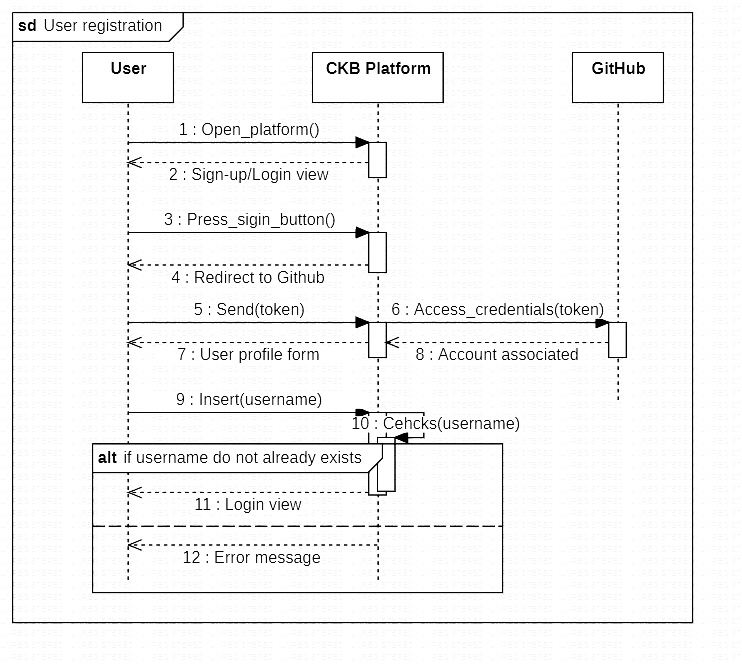
\includegraphics[width=\textwidth]{Images/User registration.jpg}
    \caption{User Registration}
    \label{fig:enter-label}
    \end{figure}

    \begin{figure}
    \item \textbf{User Login}
    \centering
    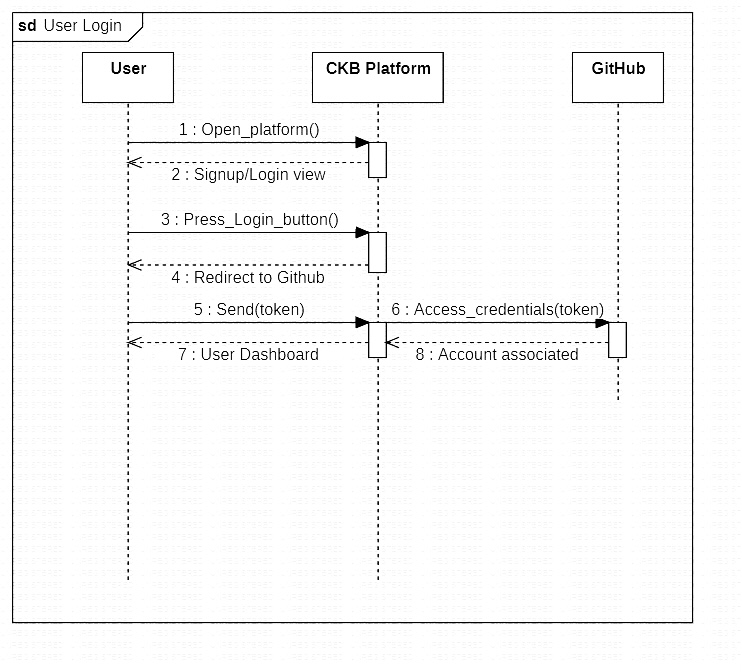
\includegraphics[width= \textwidth]{Images/User login.jpeg}
    \caption{User Login}
    \label{fig:enter-label}
    \end{figure}



    \begin{figure}
    \item \textbf{Tournament Creation}
        \centering
        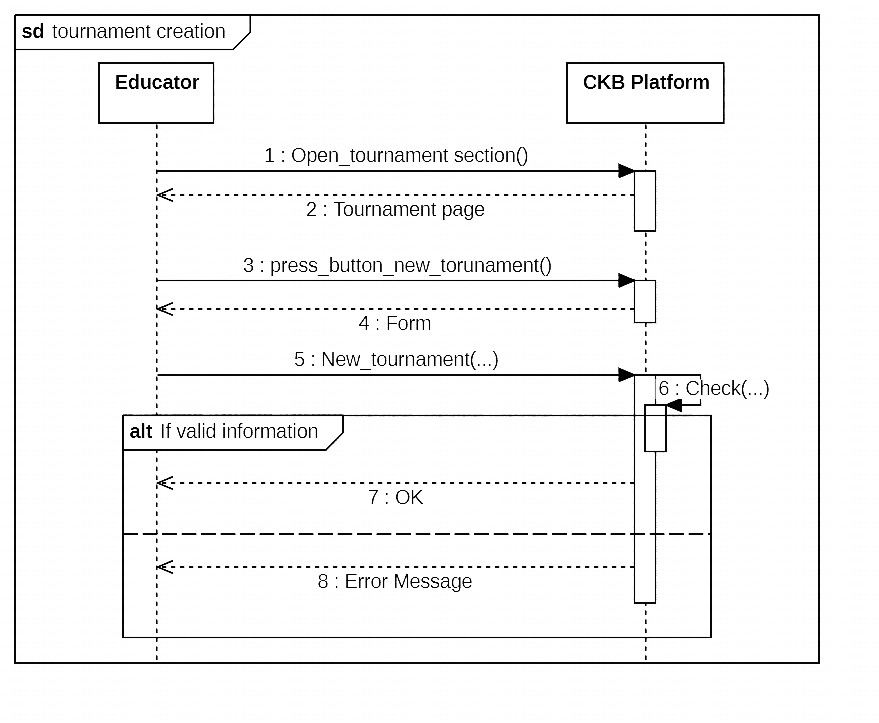
\includegraphics[width= \textwidth]{Images/Tournament creation.jpg}
        \caption{Tournament Creation}
        \label{fig:enter-label}
    \end{figure}
    
    
    \begin{figure}
    \item \textbf{Battle Creation}
        \centering
        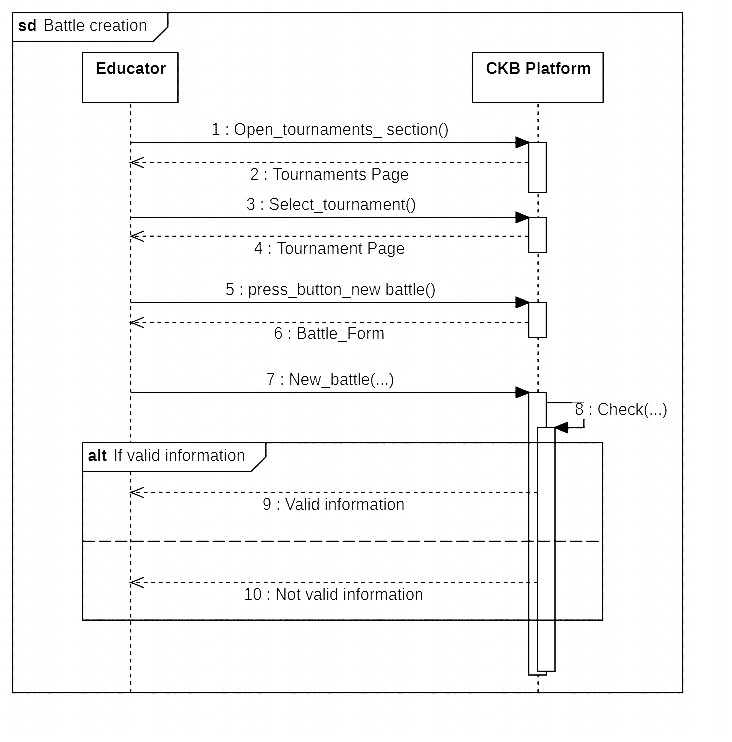
\includegraphics[width= \textwidth]{Images/Battle creation.jpg}
        \caption{Battle Creation}
        \label{fig:enter-label}
    \end{figure}
    
    \begin{figure}
    \item \textbf{Add collaborator}
        \centering
        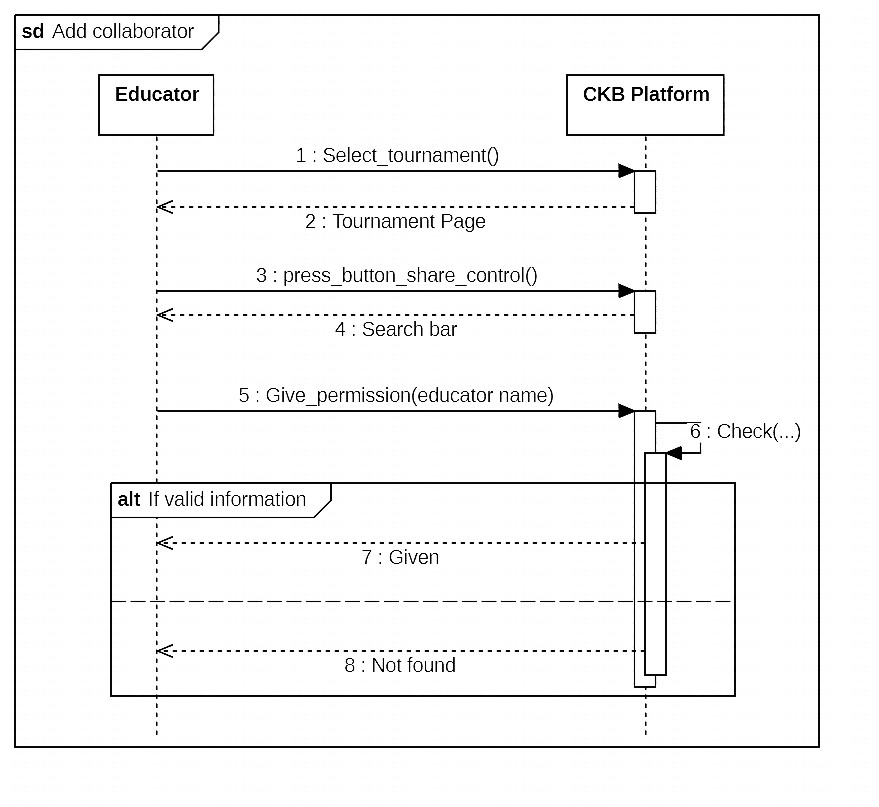
\includegraphics[width= \textwidth]{Images/Add collaborator.jpg}
        \caption{Add collaborator}
        \label{fig:enter-label}
    \end{figure}
    
    
    \begin{figure}
    \item \textbf{Team Creation}
        \centering
        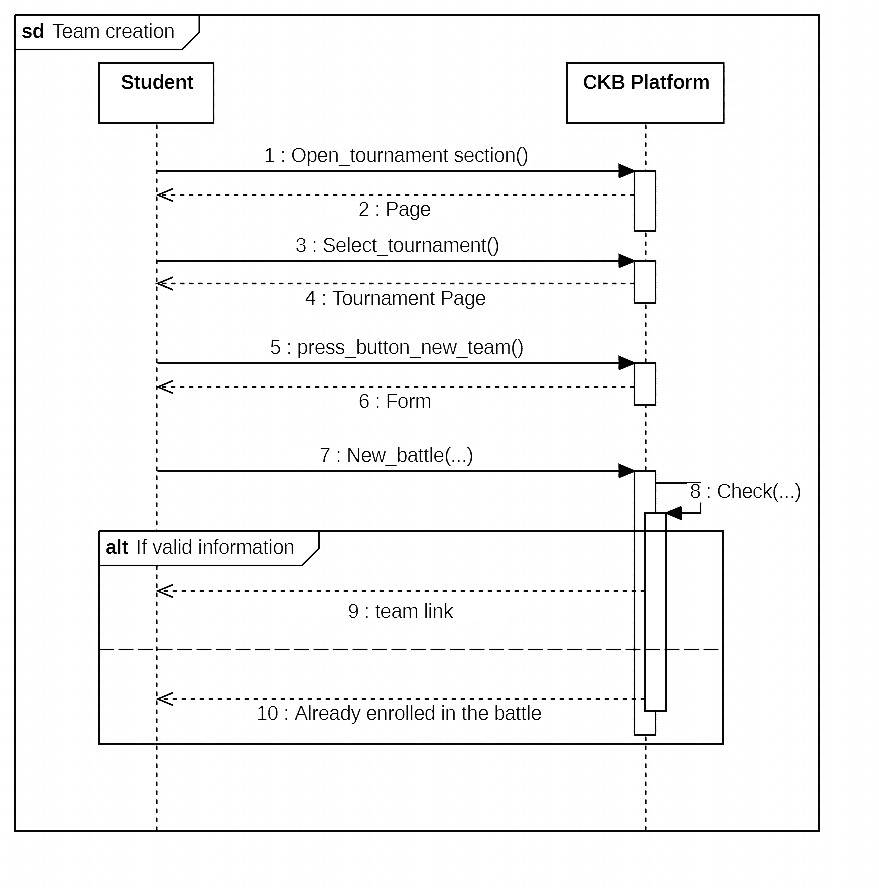
\includegraphics[width= \textwidth]{Images/Team creation.jpg}
        \caption{Team Creation}
        \label{fig:enter-label}
    \end{figure}
    
    \begin{figure}
    \item \textbf{Join Team}
        \centering
        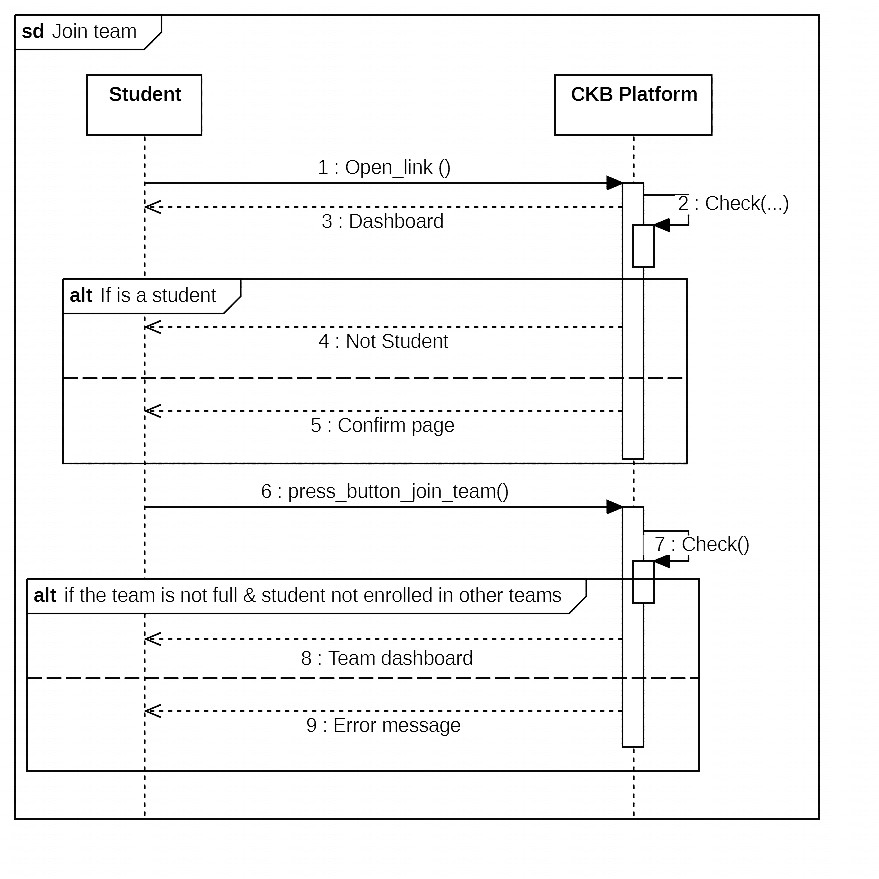
\includegraphics[width= \textwidth]{Images/Join team.jpg}
        \caption{Join Team}
        \label{fig:enter-label}
    \end{figure}
    
    \begin{figure}
    \item \textbf{Battle Begins}
        \centering
        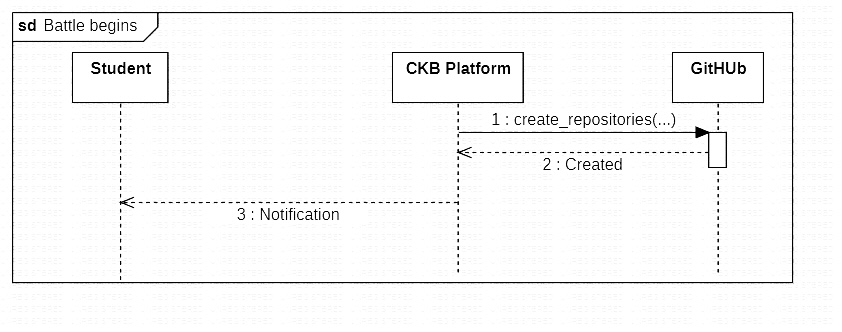
\includegraphics[width= \textwidth]{Images/Battle begins.jpg}
        \caption{Battle Begins}
        \label{fig:enter-label}
    \end{figure}
    
    \begin{figure}
    \item \textbf{Submits code}
        \centering
        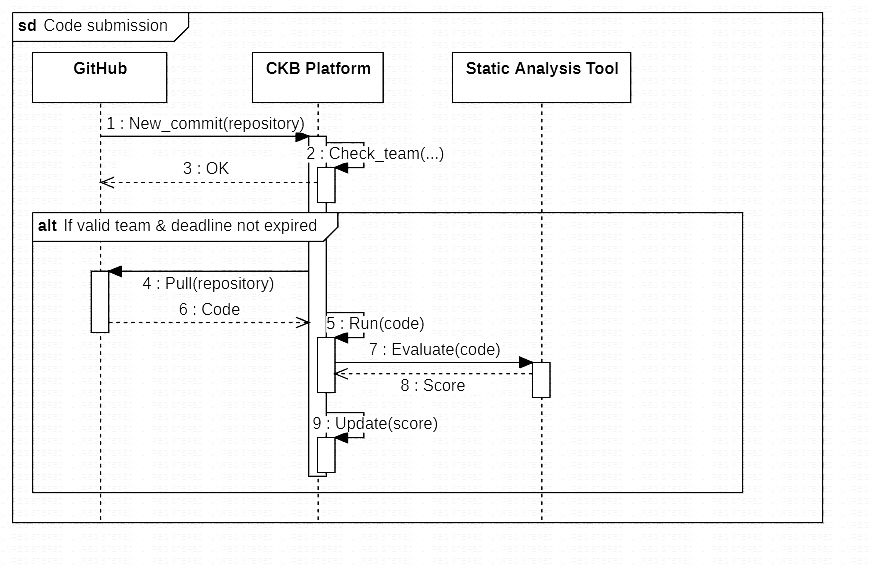
\includegraphics[width= \textwidth]{Images/Code submission.jpg}
        \caption{Submits Code}
        \label{fig:enter-label}
    \end{figure}

    \begin{figure}
    \item \textbf{The battle ends}
        \centering
        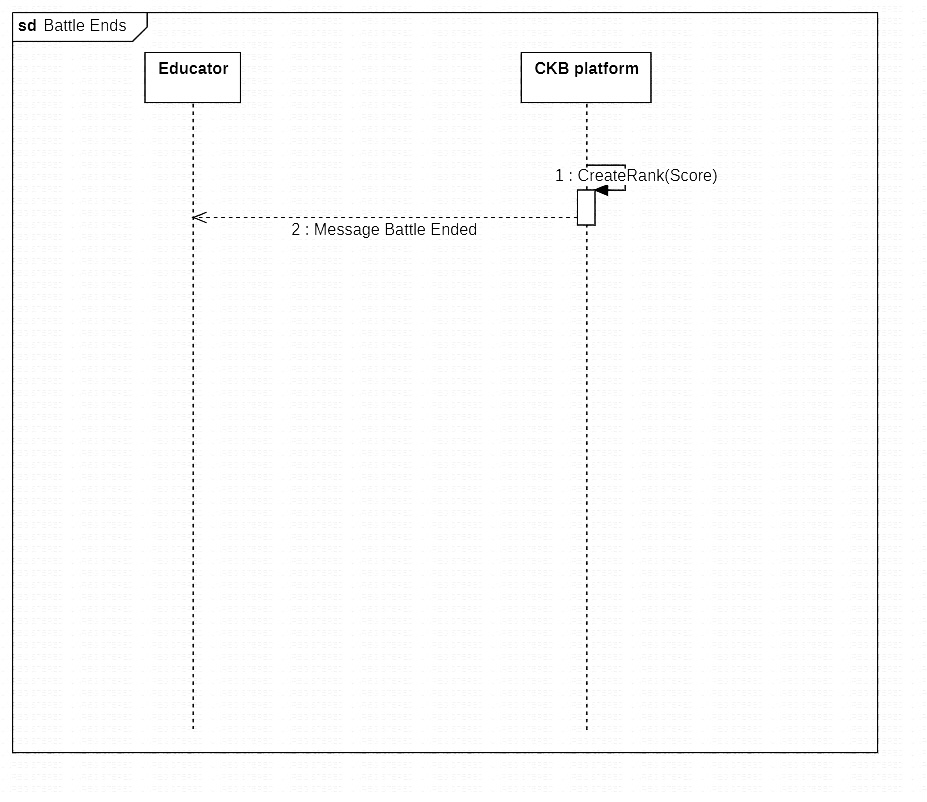
\includegraphics[width= \textwidth]{Images/Battle Ends.jpg}
        \caption{The battle ends}
        \label{fig:enter-label}
    \end{figure}
    
    \begin{figure}
    \item \textbf{Code Evaluation}
        \centering
        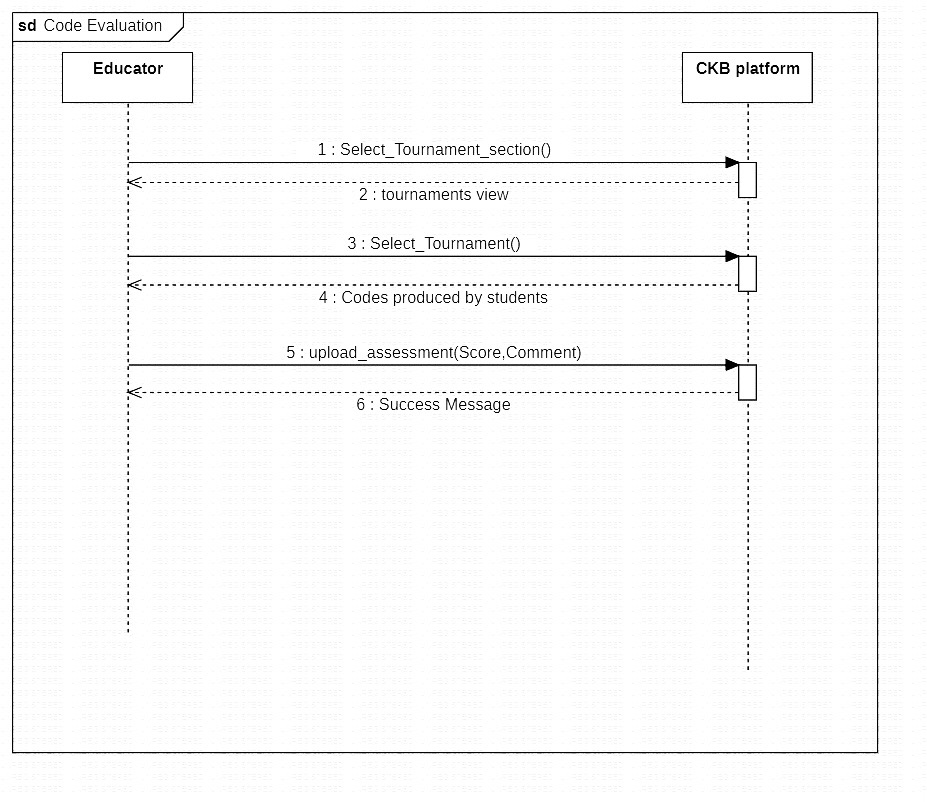
\includegraphics[width= \textwidth]{Images/f4c0a22a-3bab-4ba7-8605-08f8577774b5}
        \caption{Code Evaluation}
        \label{fig:enter-label}
    \end{figure}
    
    \begin{figure}
    \item \textbf{Publish Final Rank}
        \centering
        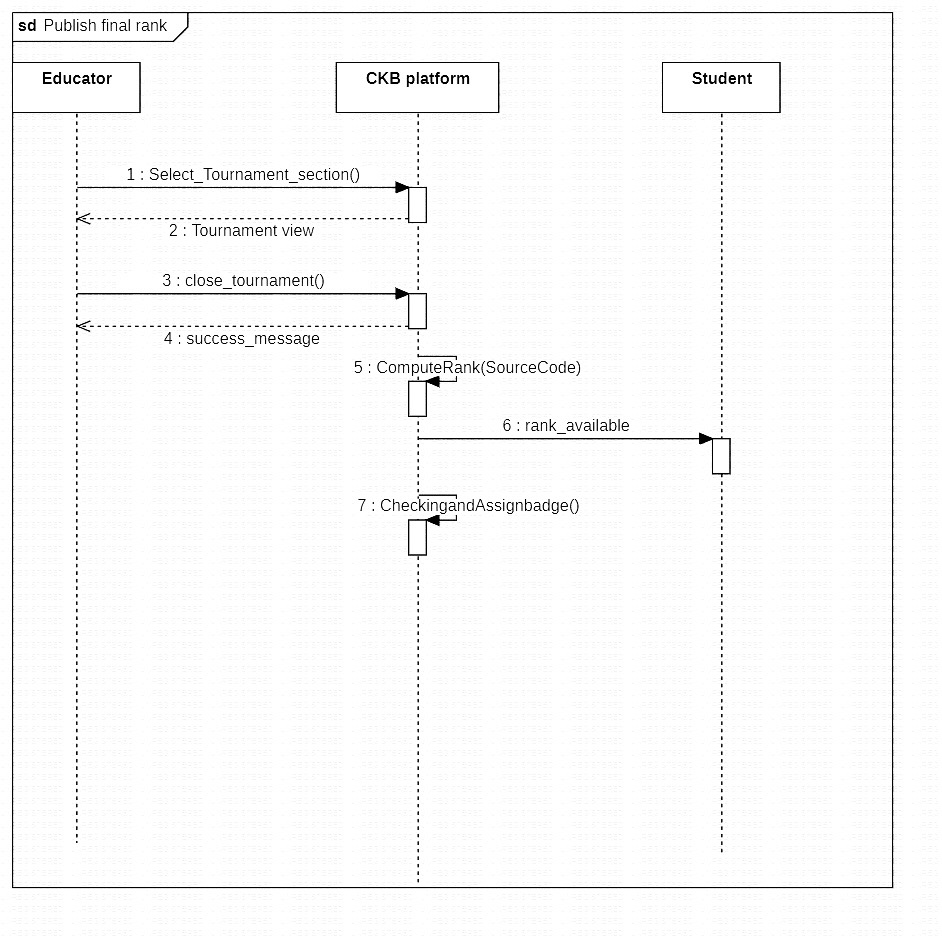
\includegraphics[width= \textwidth]{Images/e08ea53b-0385-4fb7-8284-6672fda72856}
        \caption{Publish Final Rank}
        \label{fig:enter-label}
    \end{figure}

    \begin{figure}
    \item \textbf{See Profile}
        \centering
        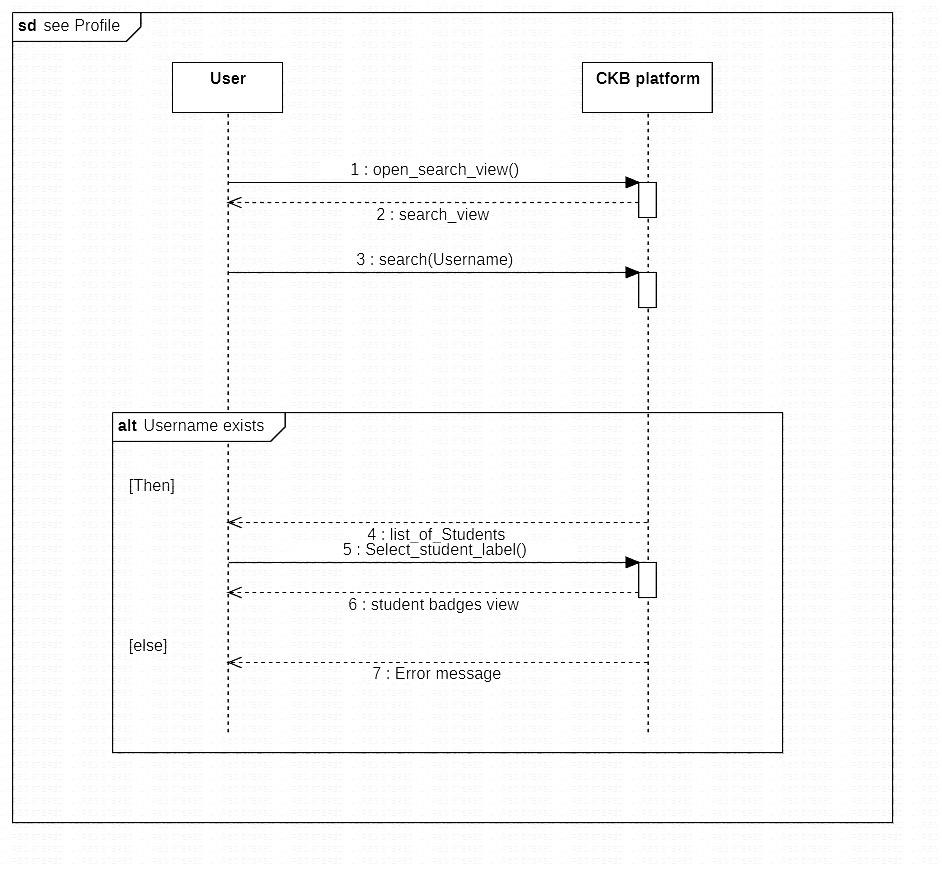
\includegraphics[width= \textwidth]{Images/WhatsApp Image 2023-12-20 at 18.34.43_e728ecf8.jpg}
        \caption{See Profile}
        \label{fig:enter-label}
    \end{figure}

    \begin{figure}
    \item \textbf{Badge Creation}
        \centering
        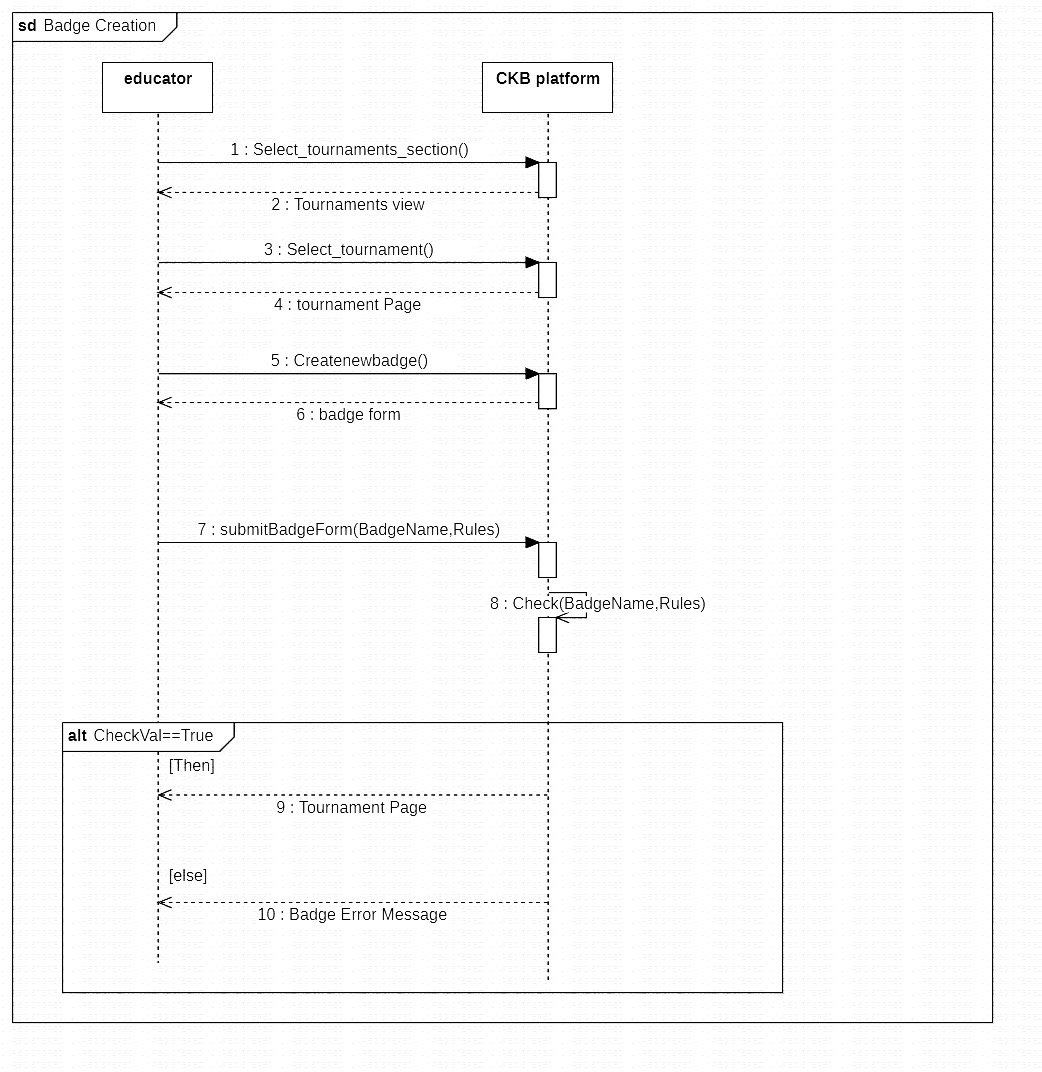
\includegraphics[width= \textwidth]{2058f325-4760-4dfa-ad83-44ce21cc7063}
        \caption{Badge Creation}
        \label{fig:enter-label}
    \end{figure}

    

    
    
\end{enumerate}








\pagebreak[4]
\newpage

\subsection{Requirement mapping}
\begin{tabular}{|p{7cm}|p{7cm}|}
\hline
\multicolumn{2}{|c|}{
\textbf{[G1] Educators create code kata battles} }
\\
\hline
\begin{itemize} 
\item [R1] The System allows users1 to register by providing their personal information (Full Name, etc.), a valid email address and a password
\item [R2] The System allows registered user to log in
\item [R3] The System allows Educators to create/modify a battle upload the code kata (description and software project, including test cases and build automation scripts)
\item [R4] The System allows to create/modify/terminate a tournament by selecting the existing battles, setting the minimum and maximum number of students per group, the registration and final submission deadline.
\item [R5] The System allows an educator to give or deny permission to his colleagues to modify a tournament.
\item [R10] The system allows educators to define the scoring criteria for a specific battle which they have permissions to
\item [R11] The system maintains and computes the scores of each battle
\item [R12] Educators can create a badge and a set of rules associated with that badge
\end{itemize}
&
\begin{itemize}
    \item [D1] User must have a reliable internet connection
    \item [D2] User personal information must be correct
    \item [D3] Educators properly insert information about a tournament
    \item [D7] The educator correctly adds information about a new badge such as new rules or badge name
\end{itemize}
\\
\hline
\end{tabular}

\pagebreak

\begin{tabular}{|p{7cm}|p{7cm}|}
\hline
\multicolumn{2}{|c|}{
\textbf{[G2] Students compete in multiple tournaments in teams} }
\\
\hline
\begin{itemize}
    \item [R1] The System allows users to register using a github acccount
    \item [R2] The System allows registered user to log in
    \item [R6] The System must notify subscribed user about upcoming battles and deadlines.
    \item [R7] The System allows students to create a team
    \item [R8] The System allows students to invite other students into one of their teams
    \item [R9] The System allows students to join a new team which they were invited
    \item [R15] The System creates a repository on GitHub containing the code kata right after the registration deadline
    \item [R16] The system sends the link to all the enrolled students after creating the repository with the code kata
    \item [R17] The System receives notifications from GitHub regarding the students registered repositories commits
    \item [R18] The System pulls the repository after receiving a notification for that repository before the deadline of that battle
    \item [R19] The System runs the appropriate test on the new code after every pull of the repository
    \item [R20] The System calculate and update the team's score for that battle after rerunning the tests
    \item [R25] The system  sends a notification about the tournament's termination to students
\end{itemize}
&
\begin{itemize}
    \item [D1] User must have a reliable internet connection
    \item [D2] User personal information must be correct
    \item [D4] The Github interaction it's reliable( the user is able to pull and push the code without losing its data)
    \item [D5] Notifications to the user must arrive as soon as the final rank is available
\end{itemize}
\\
\hline
\end{tabular}

\begin{tabular}{|p{7cm}|p{7cm}|}
\hline
\multicolumn{2}{|c|}{
\textbf{[G3] Students receive performance feedback after each battle assessment}}
\\
\hline
\begin{itemize}
    \item [R10] The system allows educators to define the scoring criteria for a specific battle which they have permissions to
    \item [R11] The system maintains and computes the scores of each battle
    \item [R12] Educators can create a badge and a set of rules associated with that badge
    \item[R13] The system assigns the badges that are created by educators as a reward for the rules they fulfill
    \item [R14] The system shows the badges that are assigned to students 
    \item [R20] The System calculate and update the team's score for that battle after rerunning the tests
    \item [R21] The system updates the personal tournament score for each student enrolled in the tournament right after the battle ends
    \item [R22] The system allows educators to manually evaluate the code after the deadline
    \item [R23] The system  allows educators to finish the consolidation stage after completely performing the manual evaluation
    \item [R24] The system computes the final ranking of the tournament immediately after consolidation finishes
\end{itemize}
&
\begin{itemize}
    \item [D4] The Github interaction it's reliable( the user is able to pull and push the code without losing its data)
    \item [D5] Notifications to the user must arrive as soon as the final rank is available
    \item [D6] The Educator properly insert an evaluation manually when it’s requested
    \item [D7] The educator correctly adds information about a new badge such as new rules or badge name
\end{itemize}
\\
\hline
\end{tabular}



\section{Performance Requirements}
The system has to guarantee good performances in order to serve a great number of users (educators and students).To achieve this goal the user experience must be as good as possible in order to fulfill this requirement the response time must be low no more than a second.If the user’s internet connection is slow the response time can increase  enormously

\section{Design Constraints}

\subsection{Standards compliance}
The CKB platform pays a great attention for what concerns users privacy cause of this the CKB project is in compliance with the  General Data Protection Regulation
(GPDR) a regulation in EU law on data protection and privacy for all
individuals within the European Union (EU) and the European Economic Area (EEA).
Moreover, the platform has to use the international format of date and time to adequate to the newer standards.
\subsection{Hardware limitations}
Here is presented a summary of the hardware features that a user should have to use the platform properly:
    \begin{enumerate}[label=\textbullet]
        \item The user must have a device with a good internet connection for providing this the device should be compatible with at least one of this standards 3G, 4G, 5G, IEEE 802.11 and  IEEE 802.3. Both for the wired and wireless communications it must be connected to a device able to guarantee an internet connection such as a modem or an access point and so on;
        \item The user must have a device with good hardware features such as a processor with high performance as an example intel i5 or i7 and a display with high resolution at least full hd and a fair amount of ram at least 8 GB.
        
    \end{enumerate}



    


\subsection{Any other constraint}
The UI should be user-friendly because the CKB platform is developed for educators and students that are learning to code. Furthermore, they must be able to use the platform in a simple and efficient way.

\section{Software System Attributes}
Here are explained some  software side attributes that the system should provide.
\subsection{Reliability}
The system has to be reliable because it will have to run continuously for a long period of time.
To ensure this feature the platform must have some sort of replication and consistency policy to avoid system crash. Moreover, as best practice, it is important to have offline backups of the system for recovering information after data loss.
\subsection{Availability}
The most important attribute that the system has to provide is the availability. The system should have an availability of 99\%.Since the platform has to achieve this goal some replication policies must be implemented and a single point of failure should be avoided. Also it has to be specially prepared for a possibly large amount of submissions when deadline is close.
\subsection{Security}
The system will store the users personal data so the security aspect must be carefully considered. Passwords stored in the central database must be encrypted.
The data store must be protected with all possible security measures to avoid internal and external attacks. The CKB platform must ensure integrity, consistency and confidentiality by using appropriate cyber-risk avoidance policies.
Additionally, because students code will be ran on the system for the dynamic analysis, a proper way to do these has to be explored making sure no malicious code can  damage the platform.
\subsection{Maintainability}The system must guarantee a good level of maintainability. The code has to be well documented. A testing routine has to be provided and it has to cover at least 75\% of the entire code excluding the UI code.
\subsection{Portability}
The system is a web application so it must be compatible with different web browser (Firefox,Google Chrome and so on) and devices (smartphones, computers, etc).





%------------------------------------------------------------------------------------------------------------------------------------------------
\clearpage
{{\chapter{Implementation, Integration and Test Plan}}}
\label{sect:plan}
\section{Overview}
In this chapter is explained how the platform that has been described will be implemented and tested. The aim of testing is to find the majority of the the bugs in the code that the working team has been generated.
Moreover a detailed description of how components inside the code are integrated will be provided (chapter 5.3).While instead in chapter 5.2 there it's presented a description of which are the most important implementation strategy used for making the project.


\section{Implementation Plan}
The aim of this section is to describe the implementation strategies that will be used to implement, integrate and test the different components. The intention is to combine the pros of the bottom-up and threads strategies.

Using a thread strategy is functional because you can make progresses visible for users and other stakeholders.it's possible to use less drivers than expected but the integration progress is more complex.

The Top-down methodology will be used this way a basic sketch will be designed and then more complex functionalities will be added as thread unit when they are validated.

This implementation strategy allows different teams to work in parallel by accomplishing different task on their own and then every unit that has been validated will be added to the whole software architecture.
\pagebreak


\subsection{Features identification}
The features to implement are described starting from the requirements.
Some requirements need the implementation of new components while instead others require only some small changes.
Here a small recap of the most important ones.

\begin{enumerate}[label={[\textbf{F\arabic*}]}]

\item \textbf{Sign-in and sign-up}

This two features are really simple to test and the test methodology is equal for both operations it's important to distinguish the two figure of educator and student because they have different privileges and different types of interaction.
\item \textbf{Creation of a Tournament and a Battle}

This feature is a core feature which has to be tested right after the sign-up and sign-in feature.
it enables the educator to create a tournament and a battle therefore it enables the other characteristics that is possible to use inside the battle.

\item \textbf{Team Creation}:

this functionality gives the possibility to a student to create its own team and this gives also the possibility to a student to enroll in a tournament and on the other hand to be able to unlock some other features such as  upload the team code and so on.

\item \textbf{Battle Management}

For what concerns the battle management this feature groups a lot of functionalities such as verifying if the battle is ended eventually additional evaluation are needed and a notification is sent when the battle has ended so the core functionalities need to be tested as specified in previous part

\item  \textbf{Code evaluation}

The code evaluation is a feature in which the system send the code uploaded by the students to the appropriate tools and this component send the score to the platform. 

\item \textbf{Tournament Consolidation}

The tournament consolidation is a feature that enables the educator to close the tournament and in the meanwhile after the end of the tournament a notification in send to students involved in the tournament
\item \textbf{Badge Creation and assignment}

This functionality is the embodiment of the system gamification so it is a core characteristic of the system. Moreover it involves both user kind of users the educator who creates a badge and the student who has it assigned. So it is compulsory to test it

\end{enumerate} 
\pagebreak
The majority the features that are listed require the interaction  between application between client and server of the application.
So the dispatcher has to be developed at the very beginning,



\section{Component Integration and Testing}
In this section it is detailed which component is implemented in every stage of the development process and how the different components are implemented and tested

\begin{enumerate}[label={[\textbf{F\arabic*}]}]

\begin{figure}[!h]
    \item \textbf{Sign-in and sign-up}

    The only part that need to be tested is the interaction of the system with the interface with github because the authentication API provided is considered reliable by definition.  
        \centering
        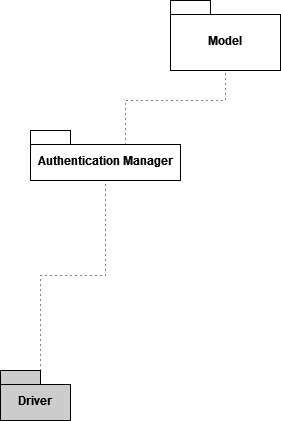
\includegraphics[width=6cm]{Images/testing.drawio(1).png}
        \caption{Sign in and Sign up developing}
        \label{fig: Sign in and Sign up developing}
       
    \end{figure}







\begin{figure}[!h]
\item \textbf{Creation of a Tournament and a Battle}

Here are added new features concerning the battles and the tournaments creation so new components and mangers need to be tested.


        \centering
        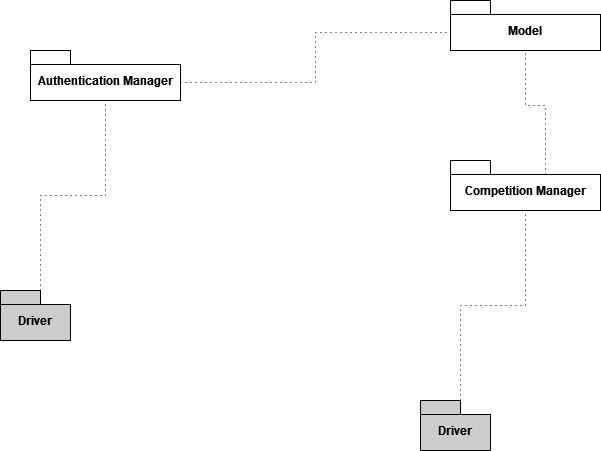
\includegraphics[width=12cm]{Images/Auth+comp.drawio.png}
        \caption{Creation of a Tournament and a Battle}
        \label{fig:Creation of a Tournament and a Battle}
       
    \end{figure}








\begin{figure}[!h]
\item \textbf{Team Creation}

Here it is explained how a team of student is created and for doing this some components are added to the previous diagram.


        \centering
        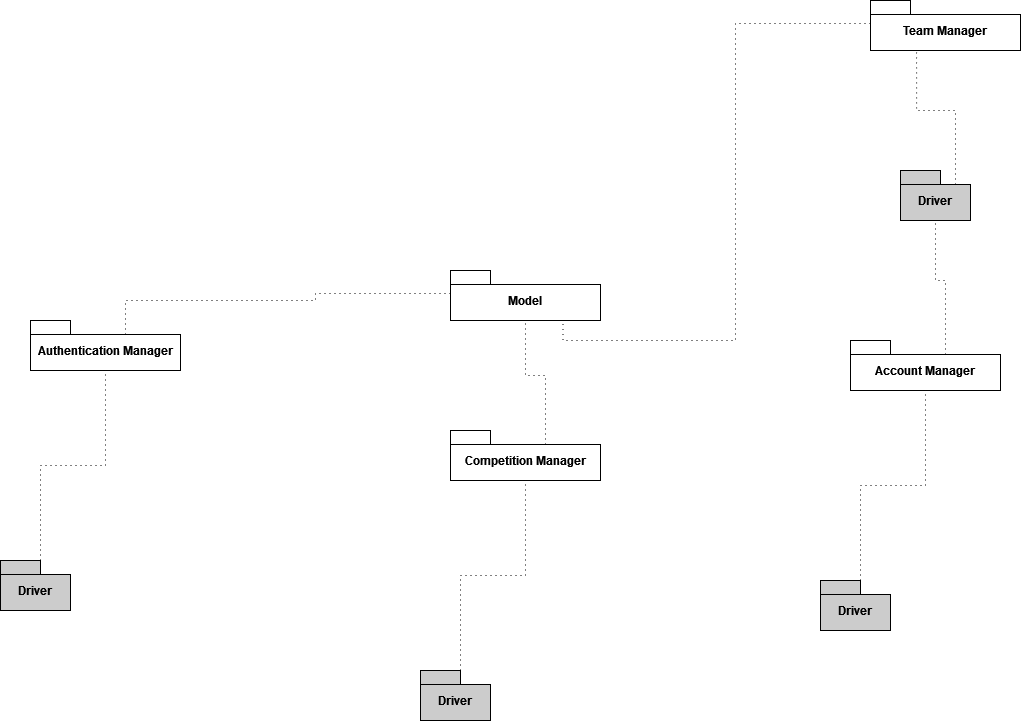
\includegraphics[width=12cm]{Images/Testing_Team_Creation.drawio.png}
        \caption{Team Creation}
        \label{fig:Team Creation}
       
    \end{figure}    

\begin{figure}[!h]
\item \textbf{Battle Management}

The battle management is managed by the Competition Manager that has been tested in a previous Diagram.The new component that has been tested is the Notification Manager important for sending notification to the different users.
         
    \centering
    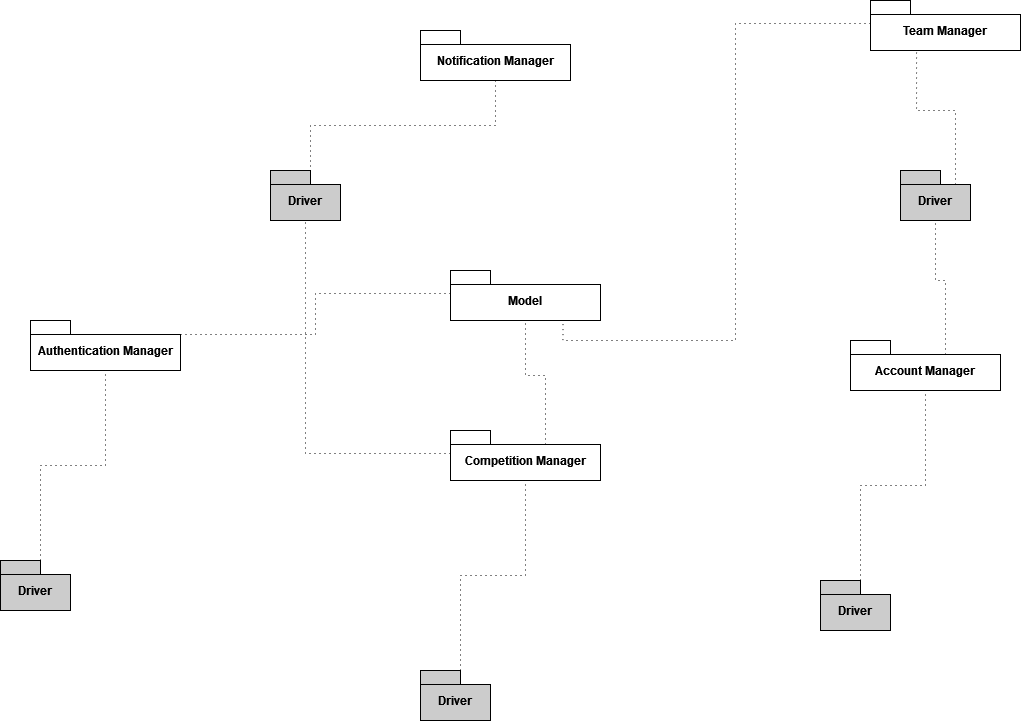
\includegraphics[width=11cm]{Images/TestingBattleManagement.drawio(2).png}
    \caption{Battle Management}
    \label{fig:Battle Management}
\end{figure}




\begin{figure}[!h]
\item \textbf{Code Evaluation}

Since the approach that has been used is the bottom-up with the combination of thread strategy the components has been added incrementally. The last component that has to be tested is the Competition Evaluation Manager which is necessary for the whole process of code evaluation and scoring but also for the submission of the codes and badge assignment.
         
    \centering
    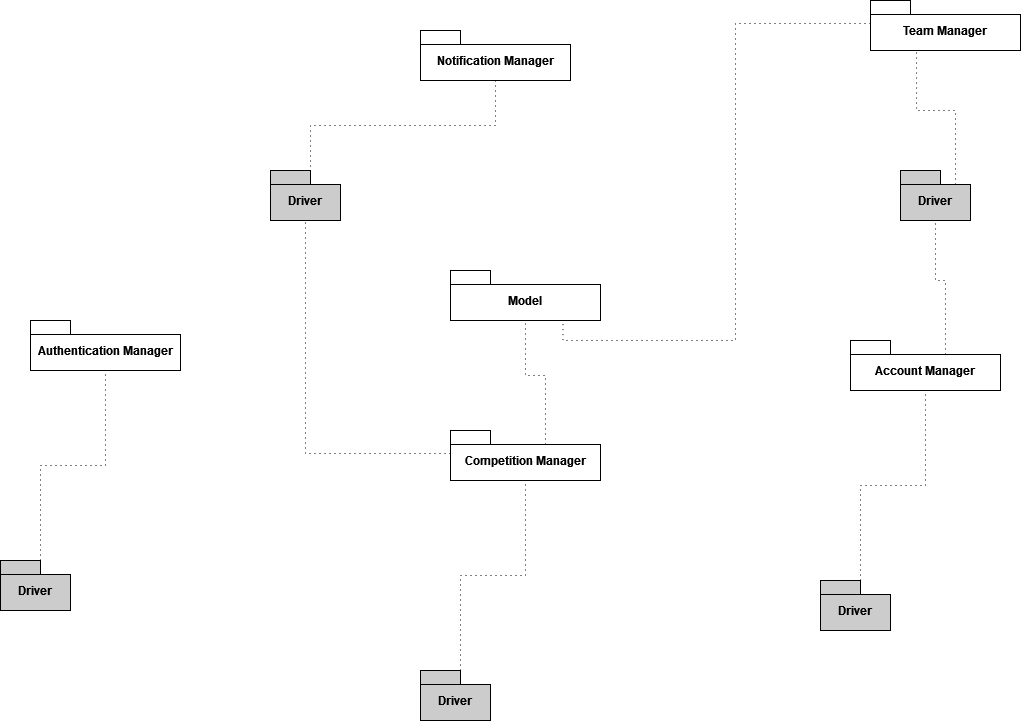
\includegraphics[width=11cm]{Images/TestingBattleManagement.drawio(1).png}
    \caption{Code Evaluation}
    \label{fig:Code Evaluation}
\end{figure}


\newpage
\item \textbf{Tournament Consolidation}

For what concerns this feature all the component has been tested in the previous diagrams.The only thing that to be tested is the piece of code in the Competition Manager that is in charge of consolidating the tournament. 

\item \textbf{Badge Creation and assignment}

The same things must be asserted for the badge creation and assignment but what has to be tested are the pieces of code that are in charge of doing this things in the respective managers    

\end{enumerate}

\newpage
\section{System testing}
CKB platform has to be tested for being sure that what the different teams coded has the correct functionalities which are consistent with what they expected to obtain.Therefore, During the development phase, each component that has been created has to be tested but not all the implemented component can be tested separately from the whole architecture so they need some stub and drivers which are helpful in replacing the missing ones.If a single thread unit has been tested and validated then it could be added to the software architecture.When the whole architecture has been coded then it could be tested entirely. The main purpose of this test is to verify if the system fulfills the functional and non-functional requirements that have been specified in the RASD document.In this process every actor that is involved in the software development is necessary so not only developers have to test the software but also the other stakeholders can contribute to the testing of the platform. The steps that will be followed during the testing are the following:
\\
\begin{itemize}
    \item \textbf{Functional Testing}:For performing this kind of test it is important to verify if the functional requirements are fulfilled.The most effecting way to achieve this test is to run the software as described in the use cases in the RASD document and verify if they are fulfilled
    \item \textbf{Performance Testing}:The main objective of this type of test is to detect bottlenecks which could affect response time, utilization, throughput, you can also detect inefficient algorithms hardware/network issues or it's possible to find out optimization possibilities.To perform this type of verification it's necessary to load the system with the expected workload and also measure and compare the performance and identify optimization possibilities
    \item \textbf{Usability Testing}: it  is a method of testing the features of a website, app, or other digital product by observing real users as they attempt to complete tasks on it.
    \item \textbf{Load Testing}:you can expose your system to some bugs such as memory leaks,buffer overflow or memory mismanagement.This type of test is useful for identifying the upper bound of components.You can also compare different architectural options.To perform this test it's compulsory to test the system with increasing workload until it can support it for a long period of time that is established before starting the test.
    \item \textbf{Stress Testing}: This test aim at verifying if the system recovers gracefully after failure. you can try increasing the system resources of you can reduce the them.
    
\end{itemize}

\pagebreak
\section{Additional specifications on testing}
During the system development it is also important to have continuous feedback from user and stakeholders.
This should happen every time a new characteristics is implemented.On the other hand during the alpha test, it is important to get the level of satisfaction of the people that are chosen for this phase for obtaining this is helpful to have the opinion of other working figure as an example psychologist, which could choose the correct question to dispense to the tester involved.  
The alpha test is also of a great importance for finding out malfunctions before the beta testing.
Beta testing is useful for real users to use a product in a production environment to uncover any bugs or issues before a general release.
The testing is important also when the application will be released because some logs should be sent to the developers that have to use them to debug



%------------------------------------------------------------------------------------------------------------------------------------------------
\clearpage
\chapter{Effort Spent}
\label{sect:effort}
In this part there is an overview of the time effort spent by each member of this team. Everyone have spent some time writing each section of this document and here its visible the amount of time.\\
\begin{itemize}
    

\item  \textbf{Andaloro Emanuele}
\begin{table}[h!]
    \centering
    \begin{tabular}{|c|p{10cm}|}
        \hline
        \textbf{chapter} & \textbf{Effort(In hours)} \\
        \hline
        1 & 5 \\
        \hline
        2 & 10\\
        \hline
        3 & 25\\
        \hline
        4 & 3\\
        \hline            
    \end{tabular}
    \end{table}

\item  \textbf{Deveali Lew Simon}
\begin{table}[h!]
    \centering
    \begin{tabular}{|c|p{10cm}|}
        \hline
        \textbf{chapter} & \textbf{Effort(In hours)} \\
        \hline
        1 & 5 \\
        \hline
        2 & 10\\
        \hline
        3 & 10\\
        \hline
        4 & 18\\
        \hline            
    \end{tabular}
    \end{table}

\item  \textbf{Galantino Claudia}
\begin{table}[h!]
    \centering
    \begin{tabular}{|c|p{10cm}|}
        \hline
        \textbf{chapter} & \textbf{Effort(In hours)} \\
        \hline
        1 & 5 \\
        \hline
        2 & 16\\
        \hline
        3 & 20\\
        \hline
        4 & 2\\
        \hline            
    \end{tabular}
    \end{table}    

\end{itemize}


%-------------------------------------------------------------------------
%	BIBLIOGRAPHY
%-------------------------------------------------------------------------

\addtocontents{toc}{\vspace{2em}} % Add a gap in the Contents, for aesthetics
\bibliography{Project_bibliography} % The references information are stored in the file named "Project_bibliography.bib"

%-------------------------------------------------------------------------
%	APPENDICES
%-------------------------------------------------------------------------


\addtocontents{toc}{\vspace{2em}} % Add a gap in the Contents, for aesthetics
\appendix
\chapter{Appendix A}
For creating the rules for the badges in a simple and extendable way, we created the following grammar:

\section{Grammar}
$<\{E,T\},\{and, or, (, ), >,\geq,<,\leq,=,-,boolean\_var,numerical\_var,$

$NUMBER\}, E, P>$

where $P$ is:

$E \rightarrow E$ ($and$|$or$) $T$ | $T$

$T \rightarrow $ ($E$) 
| ($not$)? $boolean\_var$ 
| $numerical\_var$ (>|\geq|<|\leq|=) $NUMBER$

\subsection{Examples}
Example of $boolean\_var$: PARTICIPATED\_IN\_ALL\_BATTLES

Example of $numerical\_var$: NUMBER\_OF\_COMMITS

Rule example: 

PARTICIPATED\_IN\_ALL\_BATTLES and NUMBER\_OF\_COMMITS > 0

\subsection{Parsing and evaluation}
First upon creation of the badge, the rule will be parsed to check if it is valid. Afterwards, when the tournament ends, it will be evaluated for every enrolled user with the appropriate values of all the $...\_var$ tokens.

\section{Disclaimer}
We have not established ways to create custom variables for users because it would be difficult to do so without violating encapsulation. However, we created this flexible grammar that will allow developers to easily add new variables. We will provide users with a large number of variables which will hopefully be enough, but of course any suggestion of adding new variables will be considered.

% If you need to include an appendix to support the research in your project, you can place it at the end of the manuscript.
% An appendix contains supplementary material (figures, tables, data, codes, mathematical proofs, surveys, \dots)
% which supplement the main results contained in the previous chapters.

% \chapter{Appendix B}
% It may be necessary to include another appendix to better organize the presentation of supplementary material.
\printglossary[type=\acronymtype]

% LIST OF FIGURES
\listoffigures

% LIST OF TABLES
\listoftables

% % LIST OF SYMBOLS
% % Write out the List of Symbols in this page
% \chapter*{List of Symbols} % You have to include a chapter for your list of symbols (
% \begin{table}[H]
%     \centering
%     \begin{tabular}{lll}
%         \textbf{Variable} & \textbf{Description} & \textbf{SI unit} \\\hline\\[-9px]
%         $\bm{u}$ & solid displacement & m \\[2px]
%         $\bm{u}_f$ & fluid displacement & m \\[2px]
%     \end{tabular}
% \end{table}

\cleardoublepage

\end{document}
